% !TeX spellcheck = hu_HU
% !TeX encoding = UTF-8

%----------------------------------------------------------------------------
\chapter{Gyakorlati eredmények}\label{chap:practice}
%----------------------------------------------------------------------------
Ebben a fejezetben alkalmazom a korábbiakban megismert és levezetett elméleti módszereket, megvizsgálom milyen futásidőt érnek el különböző megoldóprogramok használatával.
%, illetve összevetem az így kapott eredményeket a kombinatorikus algoritmusok hatékonyságával.

Az implementációkat a Google által üzemeltetett Colaboratory segítségével készítettem Python nyelven. A választás többek között azért esett erre a rendszerre, mert a D-Wave Systems által, Python nyelven publikált könyvtárat szerettem volna felhasználni, és ez így nem csak minimális konfigurációval megoldható, de az eredmények könnyen rekonstruálhatók a konténer technológia miatt, és nem befolyásolják őket a lokális, saját gépen eszközölt módosítások.

A teszteléshez generált gráfok előállításához és reprezentálásához a NetworkX könyvtárat használtam fel \cite{NetworkX}.

\section{QUBO-k megoldása}

A QUBO-k optimalizálásra több különböző módszert alkalmazok. A legtöbb megoldó a D-Wave által publikált könyvtárban található, de felhasználok tőlük független szoftvert is, ezzel erősítve a mezőnyt. 

\subsection{D-Wave}\label{sec:practiceDwave}

A D-Wave Ocean nevű programcsomagja több lehetőséget kínál QUBO formák megoldására. Van egzakt megoldója, ez azonban nagyon kicsi bemenetekre is használhatatlan a gyakorlatban, hiszen működési elvét tekintve, minden lehetőséget kipróbál. Ezen kívül van lehetőség kvantum számítás szimulálására, vagy egy valós kvantumgépnek is elküldhetjük a problémát a megfelelő API használatával \cite{DWaveOcean}.

Lényeges észrevétel, hogy a D-Wave megoldója -- a \refstruc{sec:QUBOform}ban leírtak szerint, az energiaminimumra törekvés elve alapján -- csak minimalizálni tud, ezért a korábban bemutatott QUBO-kat is ilyen alakra kell hozni. Ez szerencsére könnyen megy, mert ha eredetileg maximalizálni szerettünk volna, egyszerűen minden tagot $-1$-gyel kell megszoroznunk, és az így kapott függvényt minimalizálni.

A helyes konfiguráció után van lehetőségünk a korábban bemutatott QUBO modellek tényleges próbájára.

A D-Wave rendszer esetén a QUBO megadására a Python collections könyvtárának defaultdict osztályát használom, ahol kulcsként adom meg a változópárt, amelyen a kapcsolatban állnak, értékként pedig a szorzatukhoz tartozó együtthatót. Mivel elsődlegesen a D-Wave-et használom, mint megoldószoftvert, így a példakódokban is így konstruálom meg a QUBO-t, azaz, egy Q defaultdict osztályt használok.

A szimulált kvantumgépen való megoldás mellett két fő iránya van a D-Wave számítógépek használatának. Ebből az egyik a direkt módon beágyazása a problémának kvantumszámítógépre, a mások pedig egy hibrid megoldót használ, mely klasszikus optimalizációkat is végez.


A direkt QPU-t (Quantum processing unit) használatával sajnos probléma ütköztünk, ahogy nőtt a probléma mérete, nem túl nagy, vagyis pár száz csúcsot tartalmazó gráfokra is túl hosszú volt a beágyazás, és időnként túl sokat kellett kvantum erőforrásra is várni. Sajnos nem is teljesen sikerült kideríteni, hogy ennek miért van köze a probléma méretéhez, de nagyobb bemenetek esetén jellemzőbb volt ez a viselkedés. Azért is érdekes, mert a probléma megoldása a QPU-n hamar elkészül (amennyiben eljut odáig), amely kiderül a jelentésekből. Az erőforrásra várakozás azért tűnik valószínűnek, mert a kliens, ahonnan a hívást végzem többször egy \verb+get_solvers+ nevű függvény belsejében várakozik. Ugyanakkor viszont nem ez tűnik az egyetlen oknak, hiszen kisebb problémák megoldásánál nem jelentkezik ez a probléma, így azt is sejtjük, hogy a probléma beágyazása valamiért nem történik meg hatékonyan.
További probléma a direkt beágyazással, hogy a fizikai qubitek száma rendkívül korlátos. Az egyszerű maximális vágás párszáz csúcs, így logikai qubit leképezése még nem reménytelen, de a maximális K-vágásnál, mivel a változók száma rendkívüli módon kezd növekedni, és sok klikk is kialakul közben, ez már nem bizonyult használható megoldásnak. Kimondottan a dokumentációban is megtalálható egy rész, amely a óvatosságra int, ha sok változót szeretnénk használni, ahol példaként 100 csúcs gráfot hoz, amely ezek szerint a kvantum világban már sok változónak számít. (Persze ennek ellenére szomorúan szembesültünk azzal, hogy a D-Wave API semmilyen hibaüzenet vagy figyelmeztetés formájában nem adja ezt tudtunkra, hanem probléma nélkül lefut, majd gyakorlatilag egy random vágást ad vissza eredményül. Hasonlóan, mint nagy bemenetek esetén a hibrid megoldók, ahogy az kiderül a \refstruc{sec:practiceOneHot} és \refstruc{sec:practiceBinary}ban is.)


Így a D-Wave-nél alapvetően maradt a hibrid megoldó használata. Ebből kétfélét tekintek, egyik egy beépített Hybrid megoldó, mely kevés módot ad paraméterezhetőségre, illetve lehetőség van HybridWorkflowt definiálni, ahol renget beállítás segítségével tudjuk finomhangolni az algoritmusunkat.


A QUBO-kat, és általánosságban a kvadratikus programozási feladatokat persze más, klasszikus megoldóprogramokkal is megoldathatjuk. A D-Wave maga is publikál egy qbsolv nevű csomagot, melyen kvantum erőforrások használata nélkül is lehetőség van a QUBO megoldására. A dokumentáció szerint ez képes megtalálni nagy QUBO problémák optimumát, a probléma részproblémákká bontásával, miközben egy klasszikus megoldót használ, amely a tabu algoritmust futtatja \cite{DWaveOceanQbsolv}. 

\subsection{Gurobi}\label{sec:Gurobi}

Egy kereskedelmi forgalomban lévő, egyik piacvezető lineáris programozás megoldó szoftver a Gurobi, melynek bár nem fő iránya a kvadratikus programok megoldása, ezeket is támogatja \cite{gurobi}. 

Sajnos az eredmények első körben nem voltak biztatóak, viszonylag kevés változószámnál is reménytelennek tűnt egy általános QUBO megoldása, illetve nem sokkal később az ingyenes licenc korlátaiba ütköztünk, amennyiben túl sok változót szerettünk volna hozzáadni a modellhez. Az akadémia licenc igénylése kutatási célokra ugyan egyszerűen működik, ezek a licencek nem kompatibilisek konténerizált környezetekel, így a Colaboratory-ban sem használhatók. Egy viszonylag új licencelési módszer a Web License Service (WLS) használata\cite{gurobiWLS}, azonban bár a konfiguráció egyszerű, megfelelő dokumentáció hiányában, napok munkája volt ezt megfelelően elvégezni\cite{gurobiAcademicColab}.

Ha mindent jól beállítottunk, akkor például a korábban elkészített Q szótárat is átkonvertálhatjuk Gurobi modellé, és megoldhatjuk a problémát, így kapva egy QUBO megoldót. A \ref{code:solveQUBOWithGurobi}.~kódrészlet bemutatja, hogy miként tudunk egy már felépített QUBO-t megoldani, végeredményként ugyanolyan típusú look-up-table (lut)-t kapva, amelyet a D-Wave válaszából is ki tudunk nyerni. Azaz a lut i. eleme megmondja, hogy az i. változó értéke 0 vagy 1.

\begin{lstlisting}[language=python,caption=Max-cut QUBO,label=code:solveQUBOWithGurobi]	
def solveQUBOWithGurobi(Q):
	model = gp.Model('ModelFromQUBO', env=gurobiEnv)
	X = defaultdict(lambda: model.addVar(vtype=GRB.BINARY))
	expr = gp.QuadExpr()
	for ((u, v), w) in Q.items():
		expr.add(w*(X[u]*X[v]))
	
	model.setObjective(expr, GRB.MINIMIZE)
	
	model.optimize()
	
	lut = dict()
	for var in sorted(X):
		lut[var]=X[var].X
	
	return lut
	
\end{lstlisting}

Persze, érdemes észben tartani, hogy a Gurobinak nem fő profilja a kvadratikus optimalizálás, és ha lehet, akkor érdemes korlátként hozzávenni a kényszereket, ahelyett, hogy azokat a büntetőtagokként a célfüggvénybe fogalmaznánk bele. Mivel a maximális vágásnál nem voltak kényszerek, így a direkt megfogalmazás teljesen egyenértékű volt a QUBO-ból átkonvertált modellel, tehát ott semmi különbség nincs.

Viszont például \refstruc{sec:practiceOneHot}ban vizsgált maximális K-vágásnál valóban azt tapasztaltam, hogy a nyers QUBO megoldása reménytelen feladatnak tűnik a Gurobi számára, már 50-es csúcsszámnál is. Viszont amennyiben a követelményeket, hogy minden csúcs pontosan egy csoportba kerüljön, korlátként adom hozzá a modellhez, kivárható időn belül teljesít.

A Gurobi által produkált eredmények, bár pontosak, a futásidő még mindig messze elmarad a többi optimalizálótól. Azt a gyakorlati megfigyelést sikerült tennem, hogy a modell optimalizálása során viszonylag hamar megtaláljuk az optimumot, de annak belátása, hogy ez valóban az optimum, nagyon sokáig tart. 
Valójában arról van szó, hogy például egy maximalizálási folyamat során hamar megtaláljuk a primál feladat maximumát, de a duál feladat minimuma még jóval nagyobb, akár többszöröse az optimumnak, és ez csak nagyon lassan konvergál az optimum felé. Így érdemes lehet befolyásolni a megoldót, hogy ne pontos megoldást keressen, hanem megengedjük egy bizonyos hibaszázalékot. Azt a trükköt alkalmaztam, hogy egy paraméter beállításával jeleztem a megoldó felé, hogy amennyiben egy bizonyos számértéknél jobb megoldást talál, akkor termináljon a folyamat\cite{gurobiBestObjStop}. Ennek az értékét a várható optimum 0.9-szeresére állítottam be. Ezt szerencsére meg tudtam tenni, mert a gráfot úgy generáltam (\refstruc{sec:graphGeneration}), hogy előre ismerjem a várható optimumot. Ez persze egy való életbeli problémánál nem lenne megtehető, azonban akkor a D-Wave által adott eredményekre sem lenne garanciánk, hogy optimális megoldást adnak, illetve ezzel a módszerrel megkapható egy becslés, hogy mennyi ideig kell futtatni az adott algoritmust, hogy valószínűsítsük, a megoldásunk közel optimális.

\subsection{Egyéb megoldók}\label{sec:practiceOthers}

Más megoldó szoftverek kipróbálását is tervben van, de sajnos, mint kiderült lehetőségeink rendkívül limitáltak. Szóba jött például a BiqCrunch, de mivel ennek nincs Python-os API-ja, így egyelőre félretettük \cite{biqcrunch}. Ígéretesnek tűnt a qpsolvers\cite{qpsolvers}, amely egységes interfészt kínál több megoldóprogramhoz is, azonban nem támogatja az egészértékűségi kényszerek hozzáadását. További utánajárást igényel a CVXPY\cite{cvxpy} és a quadprog\cite{quadprog}, melyek akár alkalmasak lehetnek QUBO-k megoldására, eddig ezt mégsem sikerült elérni.

\section{Gráf generálása}\label{sec:graphGeneration}
Az alkalmazások ellenőrzésére speciális gráfokat generáltam, melyen így előre meg tudtam határozni a várható minimális, illetve maximális vágásokat.
A generált gráf rendelkezik négy különböző paraméterrel, ezek $N$, $K$, $p$ és $q$.
A gráfot ezek után jelöljük $G(N,K,p,q)$-val.
Az ötlet csupán annyi, hogy előre meghatározunk $K$ darab diszjunkt halmazt, hogy mindegyik csoportban pontosan $N$ darab csúcs legyen. Ezután minden élről egyénileg döntünk, hogy őt hozzávesszük-e a gráfhoz. Amennyiben egy él egy csúcs $N$-esen belül fut, ez a valószínűség legyen $q$, amennyiben két különböző csúcs $N$-es között fut, akkor legyen ez a valószínűség $p$. Világos, hogy ha $p$ kicsi, $q$ pedig nagy, akkor $K$ klasztert kapunk, ahol az élek sűrűek, a csoportok között viszont ritkák. Ellenkező esetben $K$ darab egymástól majdnem független ponthalmazt kapunk, ahol a halmazok között viszont sok él hozzá van adva a gráfhoz. Az előbbivel egy minimális vágás várhatóan a $K$ klasztert szétválasztó vágás lesz, utóbbi esetben pedig ugyanígy a maximális vágásra lesz egy jó becslésünk (\ref{code:graphGeneration}.~kódrészlet). 

Érdemes megvizsgálni az elfajuló eseteket. $G(N,K,0,1)$ esetén $K$ darab különálló egyenként $N$ csúcs teljes gráfot kapunk. $G(N,K,1,0)$ esetén pedig ennek a komplementerét kapjuk. A dolgozat keretein belül, minden közölt eredménynél egységesen a $p=0.9$ és $q=0.1$ paramétereket alkalmaztam.

Az élsúlyokat pedig egy véletlenszámmal generáltam minden élre. A gráf generáló függvényt úgy oldottam meg, hogy képes legyen bármilyen véletlenszám generátort paraméterként átvenni, de a példákban mindenhol 0 és 1 közötti egyenletes eloszlással (\ref{code:graphAddWeights}.~kódrészlet).

Érdemes észben tartani, hogy $n=|V|=N \cdot K$, tehát a kicsi $n$ és nagy $N$ nem keverendő.

\begin{lstlisting}[language=python,caption=Gráf generálása,label=code:graphGeneration]	
def createRandomGraphClusters(n, K, p, q):
	G=nx.empty_graph(K*n)
	
	#Edges across
	for k1 in range(K):
		for k2 in range(K):
			if (k1!=k2):
				for u in range(n*k1,n*(k1+1)):
					for v in range(n*k2,n*(k2+1)):
						if (random.random()<p):
							G.add_edge(u,v)
	
	#Edges within
	for k1 in range(K):
		for u in range(n*k1,n*(k1+1)):
			for v in range(u+1,n*(k1+1)):
				if (random.random()<q):
					G.add_edge(u,v)
	
	#Assign color to each node
	for k in range(K):
		for i in range(0,n):
			G.nodes[n*k+i]['c']=k
	
	return G
	
\end{lstlisting}

\begin{lstlisting}[language=python,caption=Súlyok hozzáadása gráfhoz,label=code:graphAddWeights]	
def addWeightsToGraphWithRandom(G, randAcross = random.random, randWithin = random.random):
	across_edges = [(u, v) for u, v in G.edges if G.nodes[u]['c']!=G.nodes[v]['c']]
	within_edges = [(u, v) for u, v in G.edges if G.nodes[u]['c']==G.nodes[v]['c']]
	
	for (u, v) in across_edges:
		G.edges[u, v]['weight']=randAcross()
	
	for (u, v) in within_edges:
		G.edges[u, v]['weight']=randWithin()
		
	return G
	
\end{lstlisting}

%%----------------------------------------------------------------------------
%\section{Minimális vágás}
%%----------------------------------------------------------------------------
%
%
%\subsection{Klasszikus}
%
%A probléma klasszikusan is megoldható, például folyamalgoritmus segítségével. Referenciaként a NetworkX-ben ilyen módon implementált \verb+minimum_cut+ függvényt fogom használni.
%
%\begin{lstlisting}[language=Python,caption=Min-cut flow,label=code:minCutFlow]
%	cut_value, partition = nx.minimum_cut(G, s, t, 'weight')
%\end{lstlisting}
%
%
%\subsection{QUBO}
%Egy $n$ változós bináris kvadratikus kifejezést megadhatunk tömören mátrixos formában is, ahol a $Q$ mátrix $q_{ij}$ eleme az $x_i x_j$ együtthatója. Mivel ezt a formát képes kezelni a legtöbb a megoldó, (vagy ha nem, akkor könnyen átalakítható olyan formára) ezért a továbbiakban ilyen formában adjuk meg.
%
%A minimális vágás problémája könnyen felírható QUBO-ként, ahogyan azt korábban is láttuk. Az egyetlen "trükk", hogy két speciális pontot ki kell jelölni, amelyeknek külön csoportba kell kerülniük. Mivel azonban ez a klasszikus folyamalgoritmusnál is így működik, ezért ilyen tekintetben ez a megoldás sem alsóbbrendűbb.
%
%\begin{lstlisting}[language=python,caption=Min-cut QUBO,label=code:minCutQUBO]
%	for u, v in G.edges:
%		w=G.edges[u,v]['weight']
%		Q[(u,u)]+= 1*w
%		Q[(v,v)]+= 1*w
%		Q[(u,v)]+= -2*w
%	
%	Q[(s,s)]+=P
%	Q[(t,t)]-=P
%\end{lstlisting}

%----------------------------------------------------------------------------
\section{Maximális vágás}\label{sec:practiceMaxCut}
%----------------------------------------------------------------------------

A maximális vágás klasszikus példája a QUBO-nak, ezt könnyen elintézhetjük.
%Éppen úgy működik, mint a minimális vágás, de nem szükségesek a büntető tagok.
Érdemes megfigyelni, hogy a változók száma pontosan $|V|=n$.

\begin{lstlisting}[language=python,caption=Max-cut QUBO,label=code:maxCutQUBO]
	for u, v in G.edges:
		w=G.edges[u,v]['weight']
		Q[(u,u)]+= -1*w
		Q[(v,v)]+= -1*w
		Q[(u,v)]+= 2*w
\end{lstlisting}


Az egyszerű maximális vágásra felírt QUBO-t szinte minden megoldó szoftver jól kezelte. Nagy bemenetekre is általában pontos eredményt kaptunk vissza. A leglassabb megoldónak a Gurobi bizonyult, de a képet árnyalja, hogy az ő szoftverük pontosan megkeresi az optimum értékét. Ahogyan a \refstruc{sec:Gurobi}ban már leírtam, a folyamat jelentősen gyorsítható a BestObjStop beállításával, melyet a táblázatokban és a grafikonokon \verb+Gurobi0.9+-del jelöltem.

A \refstruc{fig:maxCutQUBO} foglalja össze a különböző módszerekkel kapott futásidőket. (A tengelyeken logaritmikus skálát alkalmazok.) A futásidőknél sokszor jellemzőek voltak akár 1-2 másodperces eltérések is ugyanarra a bemenetre, a sok külső befolyásoló tényező miatt. (Kezdve csak azzal, hogy a Hibrid esetnél interneten keresztüli kommunikációval oldjuk meg a problémát, ezért csak a hálózati kommunikáció egy elég jelentős állandón változó tényező.) Kimondottan a Hybrid esetnél fordult elő többször az is, hogy időnként a futásidő kiugróan magas 1-2 perces időtartamú volt, ugyanakkora bemenetre, amelyre máskor 10-20 másodperc alatt lefutott.

Ami a \refstruc{fig:maxCutQUBO} ábrán nagyon jól látszik, hogy a sima Gurobis megoldás nagyon sok időt igénybe vett $N=1000$-nél, ami 2000 csúcsú gráfnak felel meg, már közel 1000 másodpercig tartott a lefutás. A Gurobi módosított verziója viszont a kis bemenetek $N \leq 100$ esetében a leggyorsabb volt. Ráadásul, bár csak azt írjuk elő, hogy a megoldás az optimum 90\%-ánál nagyobb legyen, így is általában megtaláljuk a pontos optimumot. (Egyedüli kivétel érdekes módon az $N=20$ esetnél fordult elő, amikor az átlagos approximációs faktor 0.93 volt.)
A bemenetek növekedésével viszont úgy tűnik, hogy a Gurobi elveszíti a versenyt, és a leggyorsabb algoritmusként a szimulált kvantumgép megoldás, és a klasszikus heurisztikus megoldó szerepel. Bár igaz, hogy ezek az algoritmusok a lokális környezeten futnak, így nincs szükség hálózati kommunikációra vagy erőforrásra várakozásra, ez akkor is meglepő eredmény. Ráadásul a grafikon alapján nem úgy tűnik, hogy ez a konstans overhead szép lassan eltűnne a bemenet méretének növekedése mellett.


\begin{figure}[!ht]
	\centering
	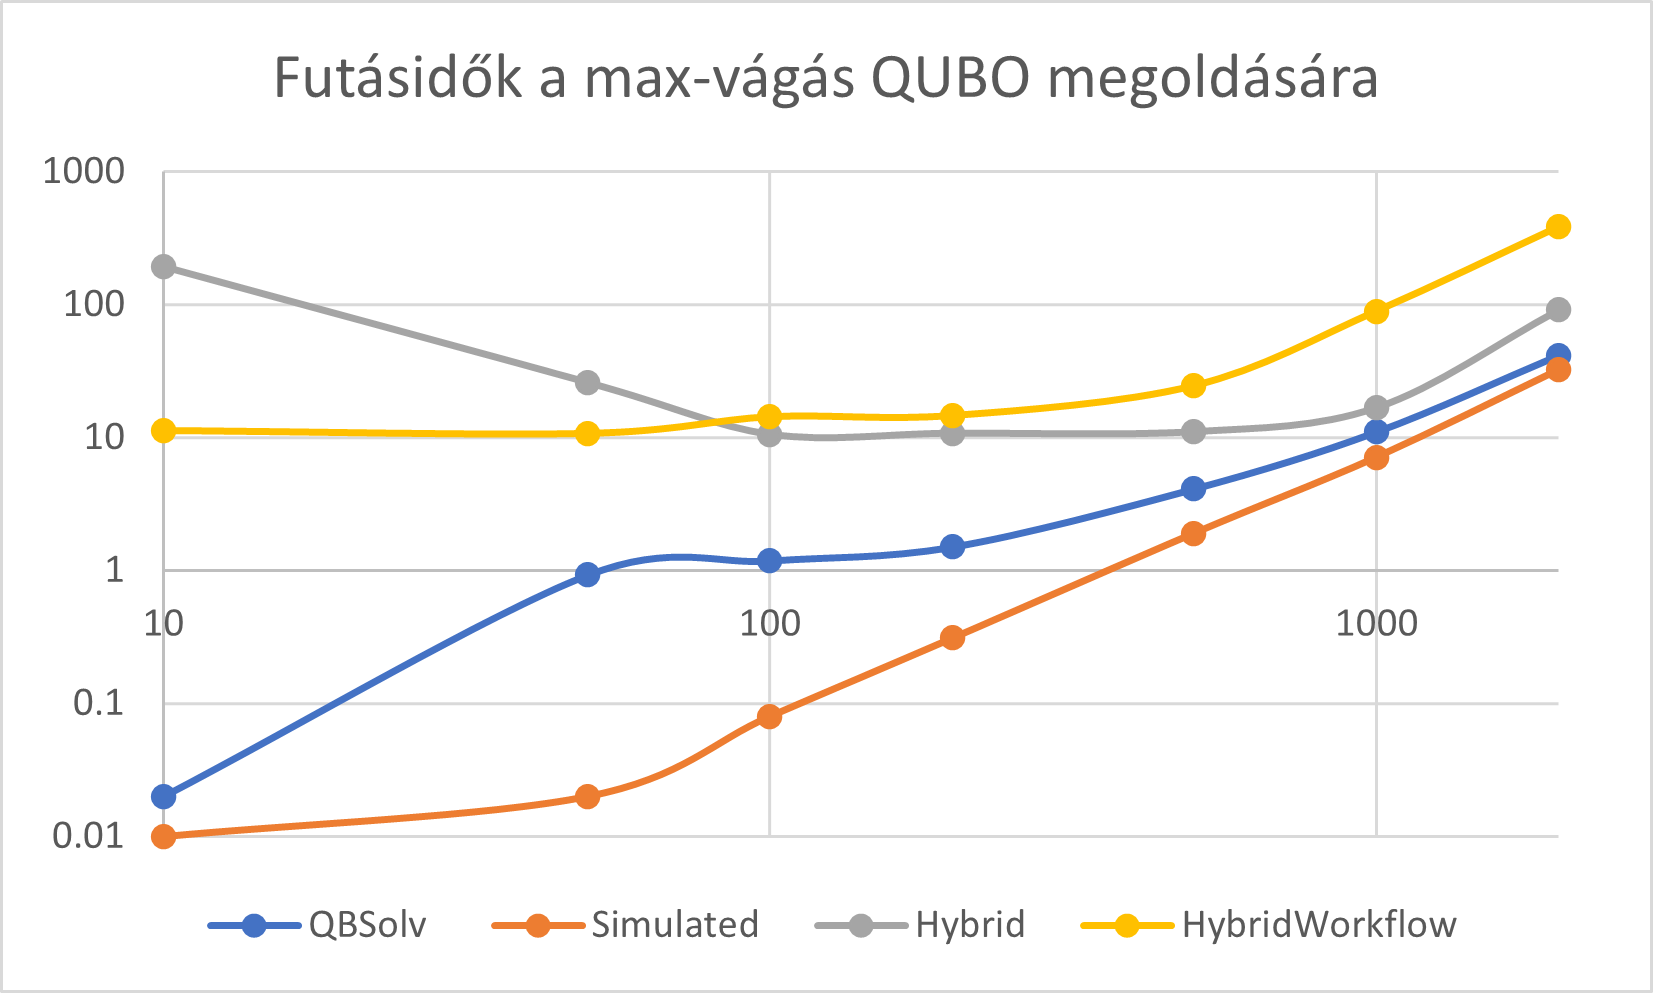
\includegraphics[width=150mm, keepaspectratio]{figures/diagrams/maxCutQUBO.png}
	\caption{Futásidők a max-vágás QUBO alakjához}
	\label{fig:maxCutQUBO}
\end{figure}

%----------------------------------------------------------------------------
\section{Maximális K-vágás (one-hot encoded)}\label{sec:practiceOneHot}
%----------------------------------------------------------------------------

\subsection{Megvalósítás}

A maximális K-vágásnál több trükköt is be kellett vetnünk. Az elméleti megfontolásokon felül, itt már csupán annyit kell még kezelni, hogy a változókat jól osszuk ki. Vagyis amíg az $x_{ui}$ változót kettő indexszel indexeltük, az elméleti felírásban, most egy indexszel kell megadnunk egyértelműen, hogy a mátrixos formába leképezhető legyen.
\footnote{Igazából ez nem szükségszerű, mert a mátrix felírásához, a Python dict típusa miatt, akár sztringeket is használhatunk kulcsként, vagyis a sor-oszlop koordináták azonosítására. Ezt a következő példában ki is használom, de ennél a feladatnál még könnyen kezelhetőek az indexek leképezése is.}
Ezt pedig úgy oldjuk meg, hogy a változókat sorba rakva blokkonként következnek az egy csúcshoz tartozó változók, azaz $x_{ui}$ az $(uK+i)$. változó lesz. Ennek megfelelően használjuk tehát az indexeket.

Ebből következik továbbá az a korábbi, de fontos megfigyelés is, hogy a változók száma itt $n \cdot K = N \cdot K^2$.

\begin{lstlisting}[language=python,caption=Max-K-cut QUBO (szimmetrikus mátrix), label=code:maxKCutQUBOSymmetric]
for u, v in G.edges:
	for i in range(K):
		for j in range(K):
			if (i!=j):
				w=G.edges[u,v]['weight']
				Q[(u*K+i,v*K+j)] += -1*w

for u in range(K*N):
	for i in range(K):
		for j in range(K):
			if (i!=j):
				Q[(u*K+i,u*K+j)] += P 
\end{lstlisting}

\begin{lstlisting}[language=python,caption=Max-K-cut QUBO (háromszög mátrix),label=code:maxKCutQUBOTriangle]
for u, v in G.edges:
	for i in range(K):
		for j in range(i+1, K):
			w=G.edges[u,v]['weight']
			Q[(u*K+i,v*K+j)] += -1*w
			Q[(v*K+i,u*K+j)] += -1*w

for u in range(K*N):
	for i in range(K):
		for j in range(i+1, K):
			Q[(u*K+i,u*K+j)] += P
\end{lstlisting}


A Gurobi használata során figyelembe vettem, hogy a korlátok célfüggvénybe való beleerőltetése nem előnyös (\refstruc{sec:Gurobi}) ezért a Gurobit nem csak a nyers QUBO megoldására használtam, hanem felhasználtam a korlátokat külön hozzáadva, és csak a ténylegesen optimalizálandó részeket célfüggvényként megadva (\ref{code:maxKCutGurobi} kódrészlet). Több mérés is azt igazolja, hogy ez a módszer sokkal jobban teljesít, mint az egyszerű QUBO megoldása (\refstruc{fig:maxKCutQUBO_K2}).

\begin{lstlisting}[language=python,caption=Max-K-cut QUBO (háromszög mátrix),label=code:maxKCutGurobi]
  model = gp.Model('MaxKCut', env=gurobiEnv)

	X = model.addVars(len(G)*K, vtype=GRB.BINARY, name="Set")
	
	#Every node can be only in one group
	for u in range(len(G)):
		expr = gp.LinExpr()
		for i in range(K):
			expr.add(X[u*K+i])
			model.addConstr(expr == 1)
	
	expr = gp.QuadExpr()
	for u, v in G.edges:
		for i in range(K):
			for j in range(i+1, K):
				w=G.edges[u,v]['weight']
				expr.add(w*X[u*K+i]*X[v*K+j])
				expr.add(w*X[v*K+i]*X[u*K+j])
	
	model.setObjective(expr, GRB.MAXIMIZE)
\end{lstlisting}

\subsection{Eredmények}


A maximális K-vágásra a futásidőket szemlélteti a \ref{fig:maxKCutQUBO_K2} és a \refstruc{fig:maxKCutQUBO_K4}. Előbbhez $K=2$, utóbbihoz $K=4$ van beállítva paraméterként. Általános tapasztalat a grafikonoknál, hogy a Gurobi mellett -- amelyet immár nem is klasszikus értelemben QUBO megoldásra használok, mert hozzáadok változókat is a modellhez --, a \refstruc{sec:practiceMaxCut}hoz hasonlóan lokálisan futó algoritmusok futnak le gyorsabban.

A \ref{fig:maxKCutQUBO_K4} grafikonon kimondottan érdekesnek tűnik, hogy a Gurobival történő megoldás hamar belassul, így összehasonlíthatatlanul rossz lesz a többi solver-hez képest. Az eredmények valóban összehasonlíthatatlanok, de sajnos más okból kifolyólag.

\begin{figure}[!ht]
	\centering
	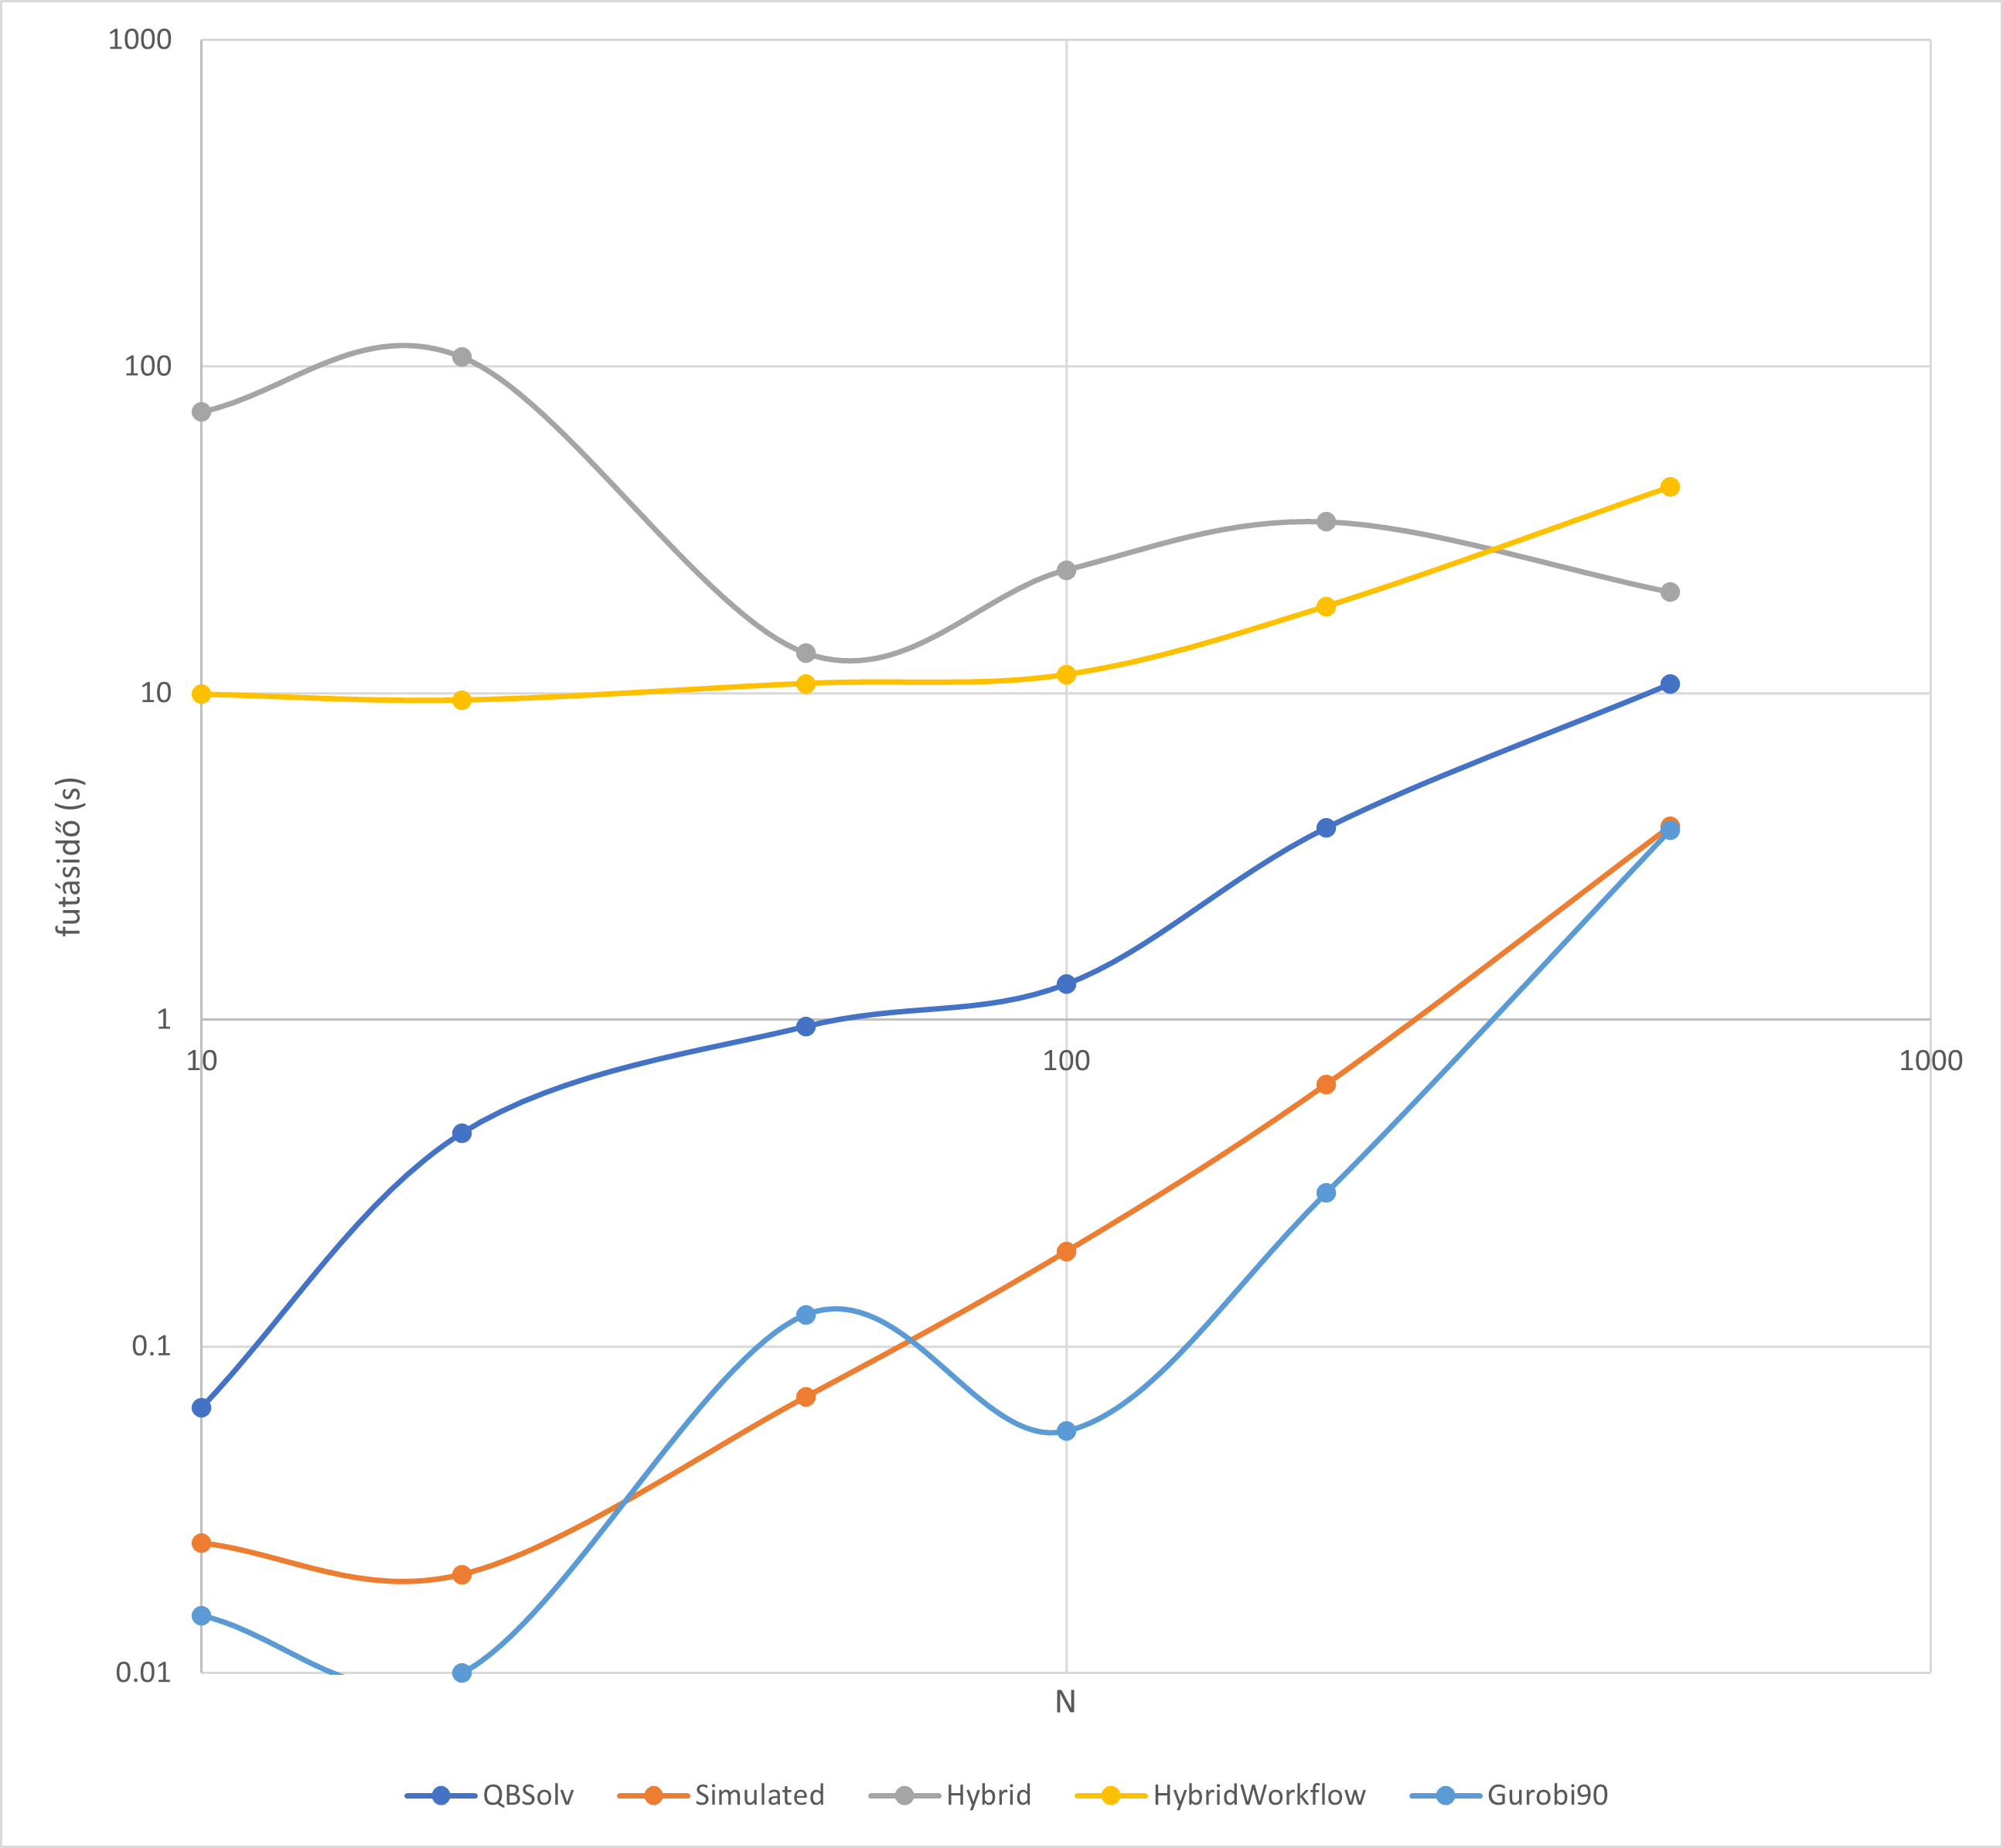
\includegraphics[width=150mm, keepaspectratio]{figures/diagrams/maxKCutQUBO_K2.png}
	\caption{Futásidők a max-K-vágás QUBO megoldására (K=2)}
	\label{fig:maxKCutQUBO_K2}
\end{figure}

\begin{figure}[!ht]
	\centering
	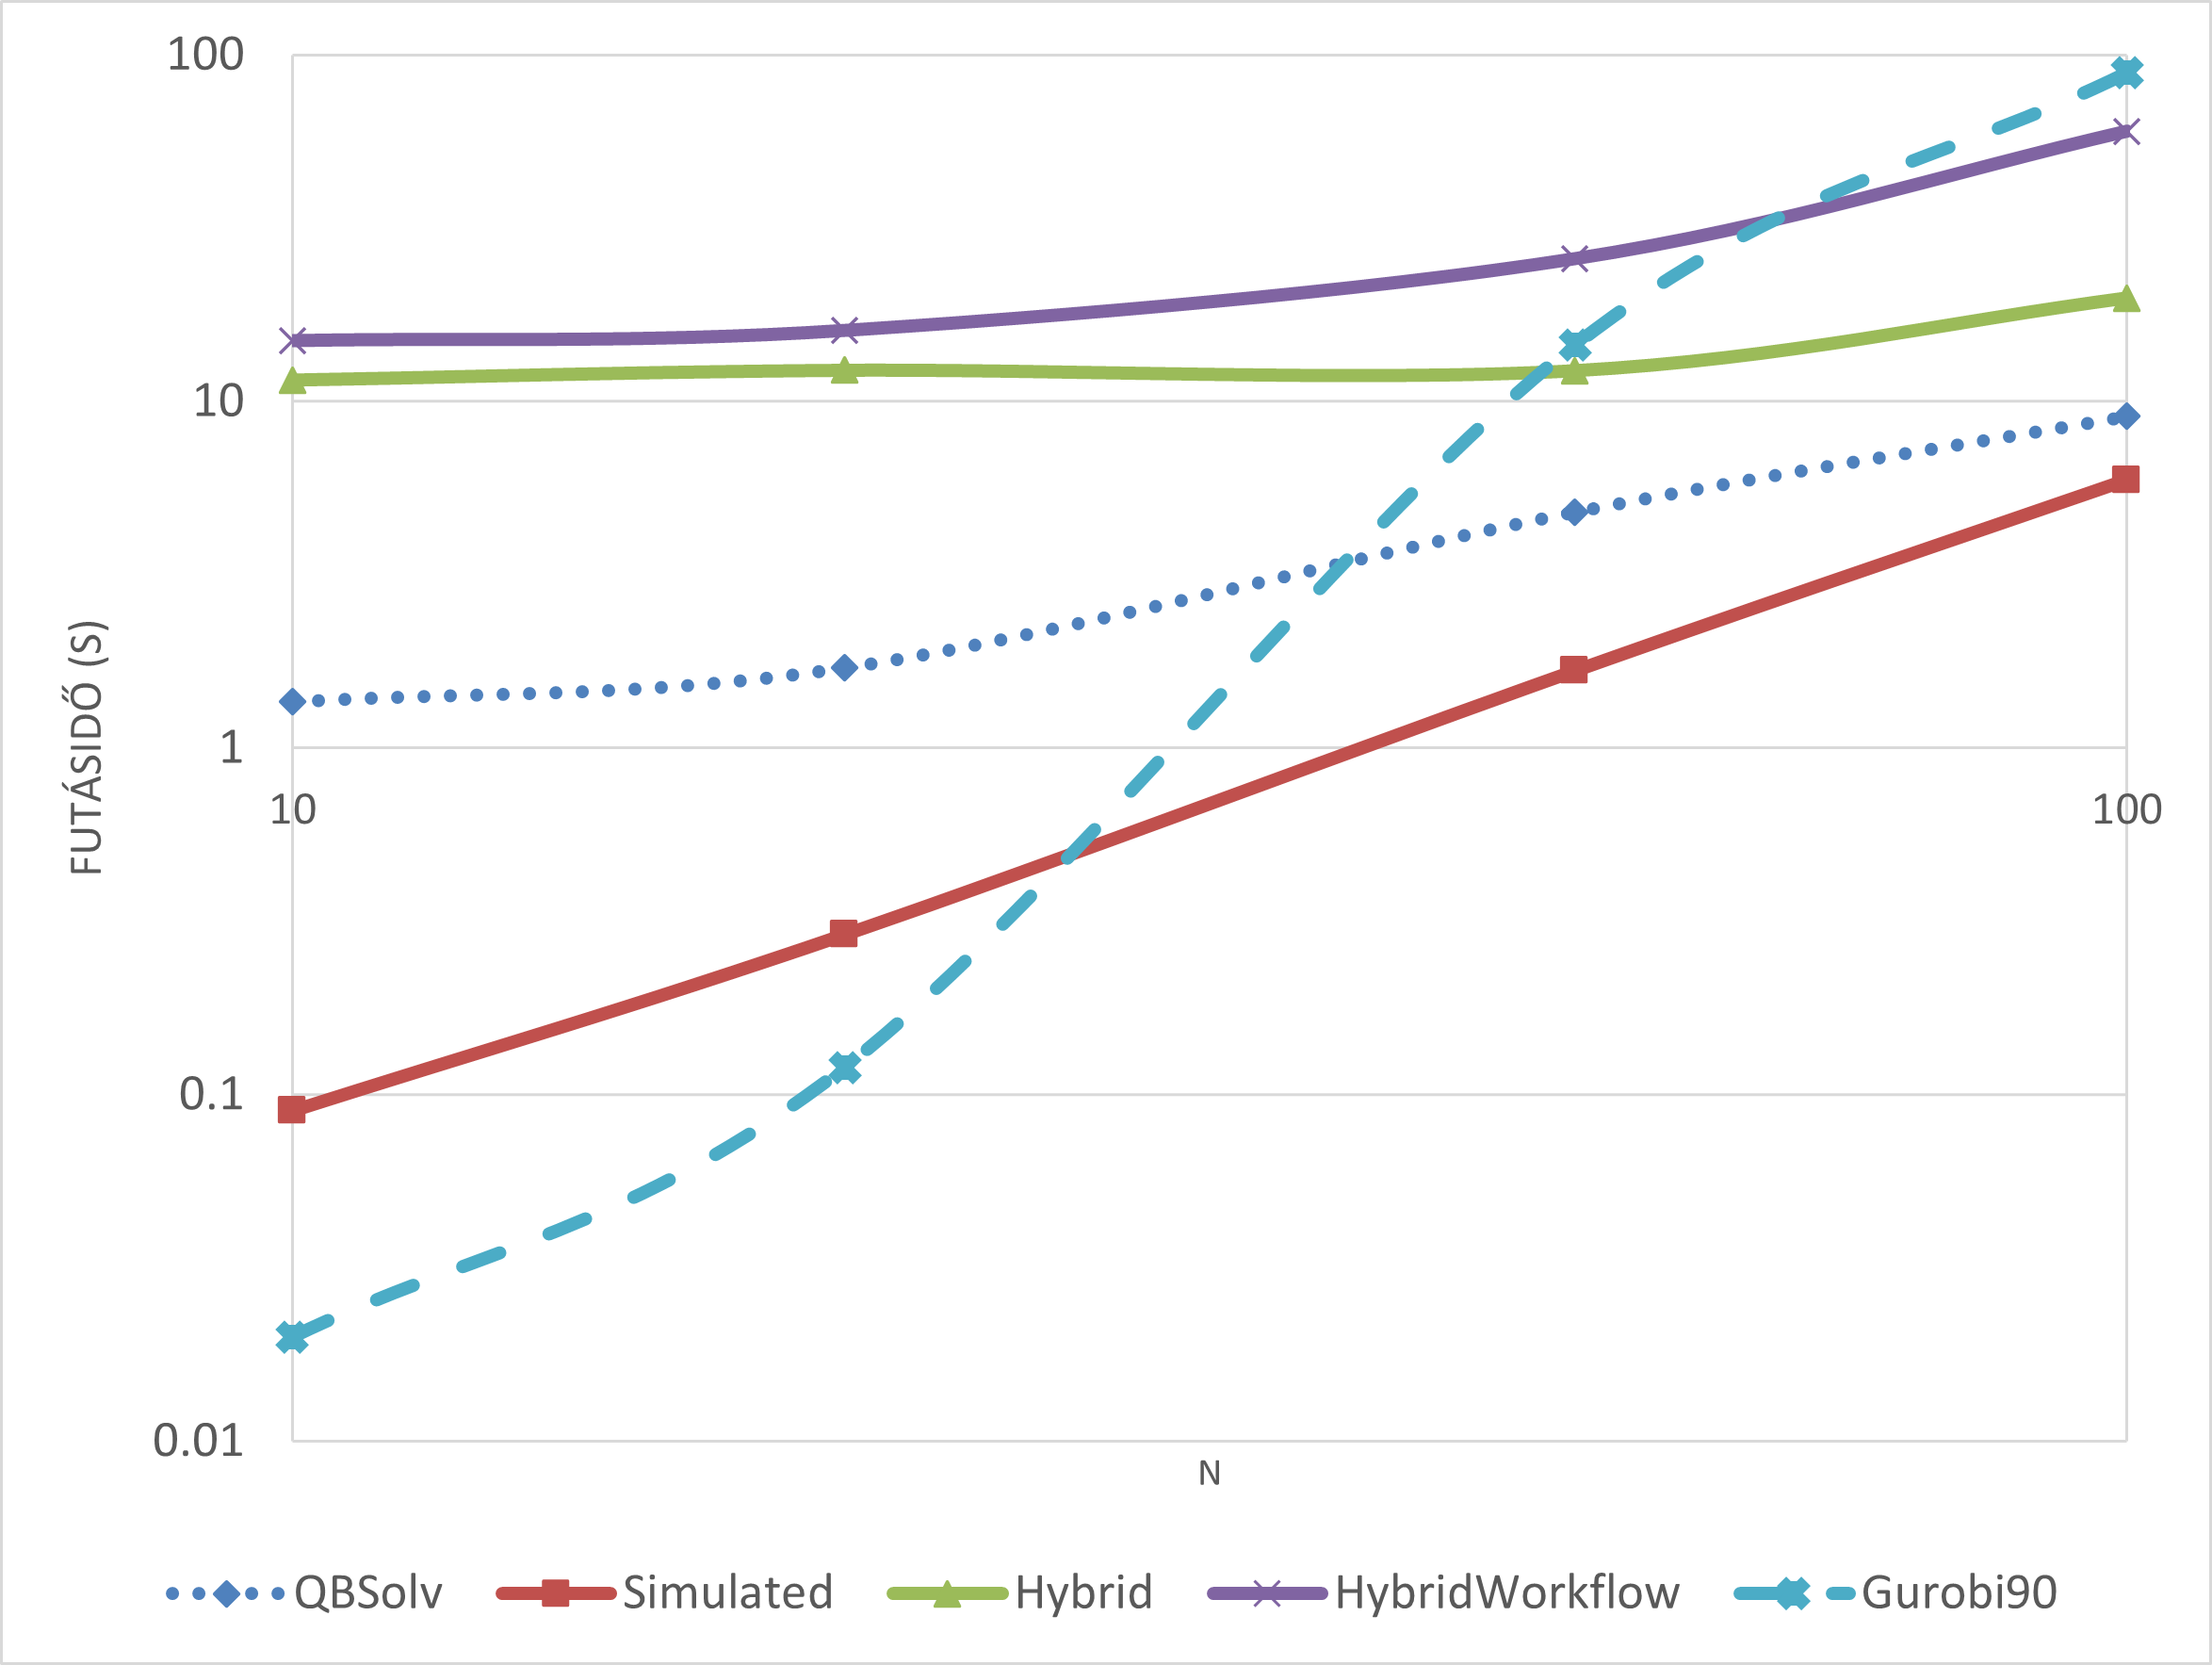
\includegraphics[width=150mm, keepaspectratio]{figures/diagrams/maxKCutQUBO_K4.png}
	\caption{Futásidők a max-K-vágás QUBO megoldására (K=4)}
	\label{fig:maxKCutQUBO_K4}
\end{figure}

Sajnos a futási idők elemzése önmagában nem elég, fontos megvizsgálni, hogy valóban jó (közelítő) eredményeket kaptunk-e. Amíg az egyszerű maximális vágásnál (\refstruc{sec:practiceMaxCut}) mindig közel jó eredményt kaptunk, és inkább a futásidő volt a szűkös erőforrás, addig a K-vágásnál gyakran kaptunk viszonylag rossz közelítéseket is, ezért érdemes mindig figyelni a talált megoldás és a várt optimum arányát, melyre továbbiakban approximációs faktorként is hivatkozok. Amennyiben ez a szám $1.0$, az azt jelenti, hogy a keresett vágást pontosan megtaláltuk.

A vágások várható optimumát könnyen megmondhatjuk a generált gráfok alapján, de nagyságrendileg is érdemes kiszámolni. Ha $p=1, q=0$ közelítést használjuk, akkor $N \approx (N-1)$ miatt, expliciten kiszámolható a \ref{goodcut} képlettel, ahol $E(W)$ az élsúlyok várható értéke.

\begin{align}
	\begin{split}
		\binom{K}{2} \, N^2 \, E(W) \label{goodcut}		
	\end{split}
\end{align}

Érdemes utánagondolni, hogy mekkora az a közelítés, amely jónak mondható, vagy másképpen, mennyi legyen legalább az a megtalált megoldás, hogy az egyértelműen jobbnak titulálható legyen, mint egy teljesen véletlen vágás. Erre persze a válasz nem egyértelmű, de a nagyságrendek elhelyezését megkönnyítendő, érdemes kiszámolni egy teljesen véletlen vágás approximációs faktorát. Egy véletlenszerű vágás, amikor a $K$ csoport mindegyikébe, minden eredeti csoport $K$-ad részét tesszük. Ekkor ha ismét a $p=1, q=0$ közelítést használjuk akkor kiszámolhatjuk az élek számát, amelyet még szorozni kell az élsúlyozás várható értékével, így kapjuk a \ref{badcut} szerinti formulát. 

\begin{align}
	\begin{split}
		K \, \frac{N}{K} \, \left( N-\frac{N}{K} \right) \, \binom{K}{2} \, E(W) = \label{badcut} \\
		 N^2 \, \left( 1 -\frac{1}{K} \right) \,\binom{K}{2} \, E(W)
	\end{split}
\end{align}

A \ref{badcut} formulát osztva a \ref{goodcut} kifejezéssel, megkapjuk a \ref{approxcut}-ot, mint várható legrosszabb approximációs faktort.

\begin{align}
	\begin{split}
		\left( 1 -\frac{1}{K} \right) \label{approxcut}
	\end{split}
\end{align}

Vagyis $K=2$ esetben legalább $0.5$ felett lesz az arányszám, amíg például $K=4$ esetben legalább $0.75$. Ezt fontos szem előtt tartani, hiszen ez azt jelenti, hogy $K=4$ esetben egy $0.8$ approximációt elérő algoritmus egyáltalán nem nevezhető jónak, hiszen alig jobb, mintha a gráfnak egy random felosztását adnánk vissza eredményül.

A \refstruc{fig:maxKCutQUBO_K2approx} és \refstruc{fig:maxKCutQUBO_K4approx} szemlélteti a megoldások pontosságát. Láthatjuk, hogy $K=2, N \leq 200$ esetre minden esetben megtaláltuk az optimumot, bármely optimalizálót is használjuk. Sajnos viszont $N=500$, illetve $K=4$ esetben már gyakorlatilag használhatatlanul rossz vágásokat kapunk vissza. A problémával nagyon sokat foglalkoztam, így a hibakeresés során a kapott felosztáson ,,szemmel végignézve" is konstatálhattam, hogy valóban, mintha véletlen felosztásról lenne szó.

\begin{figure}[!ht]
	\centering
	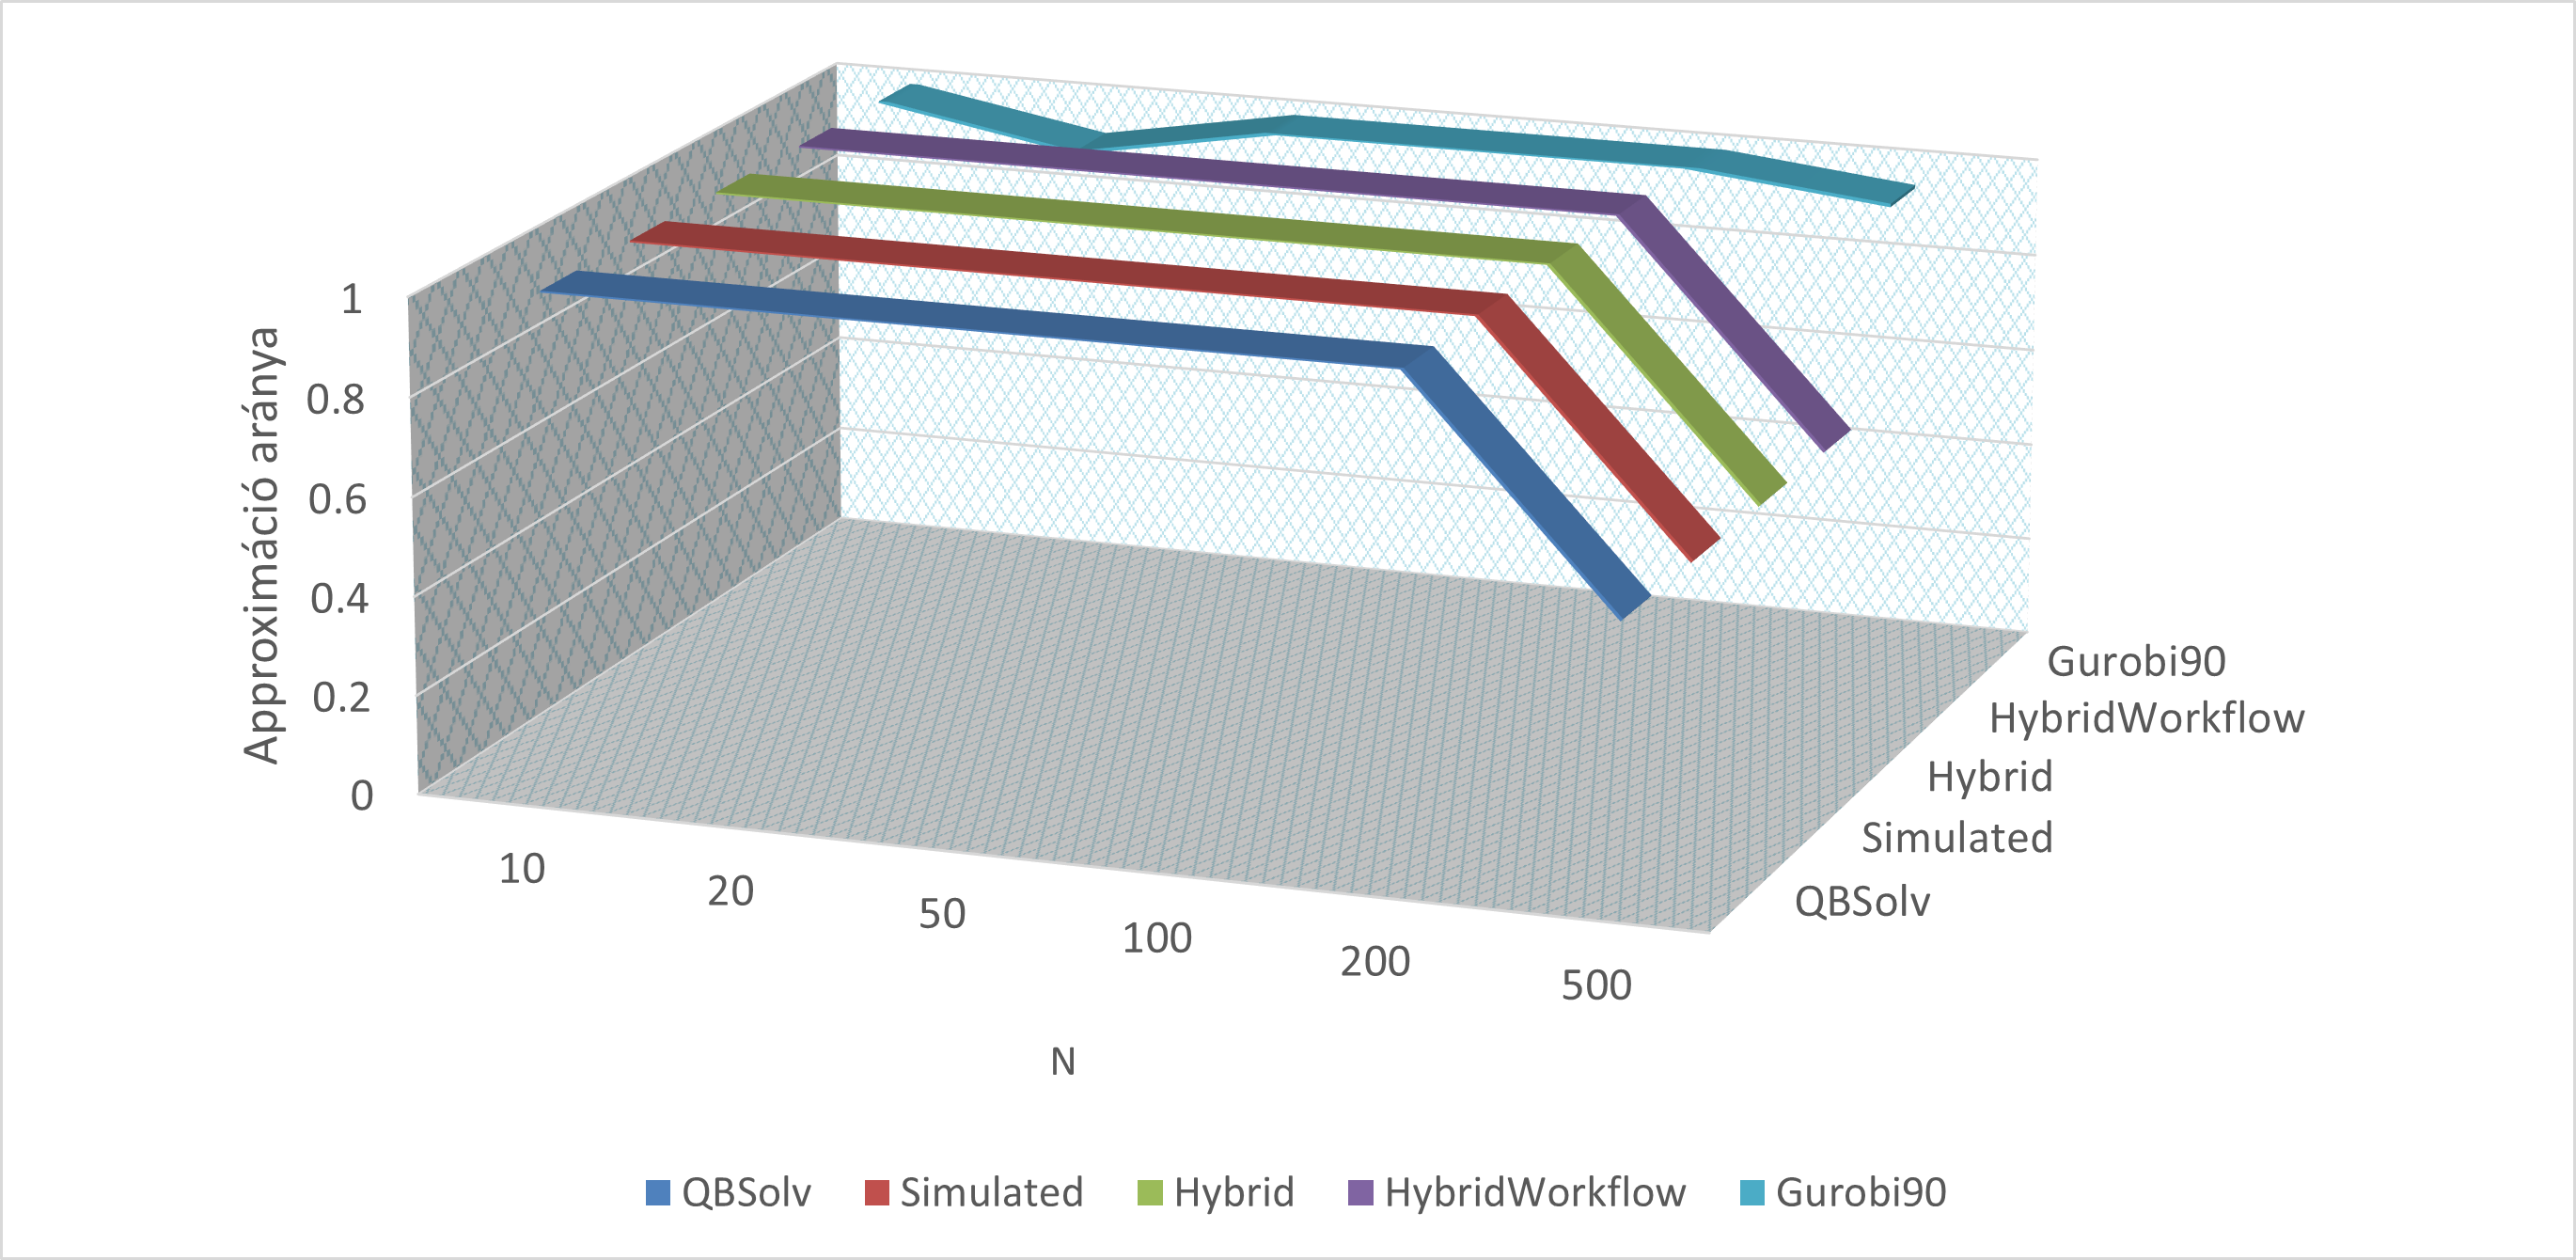
\includegraphics[width=150mm, keepaspectratio]{figures/diagrams/maxKCutQUBO_K2approx.png}
	\caption{Approximációs faktorok a max-K-vágás QUBO megoldására (K=2)}
	\label{fig:maxKCutQUBO_K2approx}
\end{figure}

\begin{figure}[!ht]
	\centering
	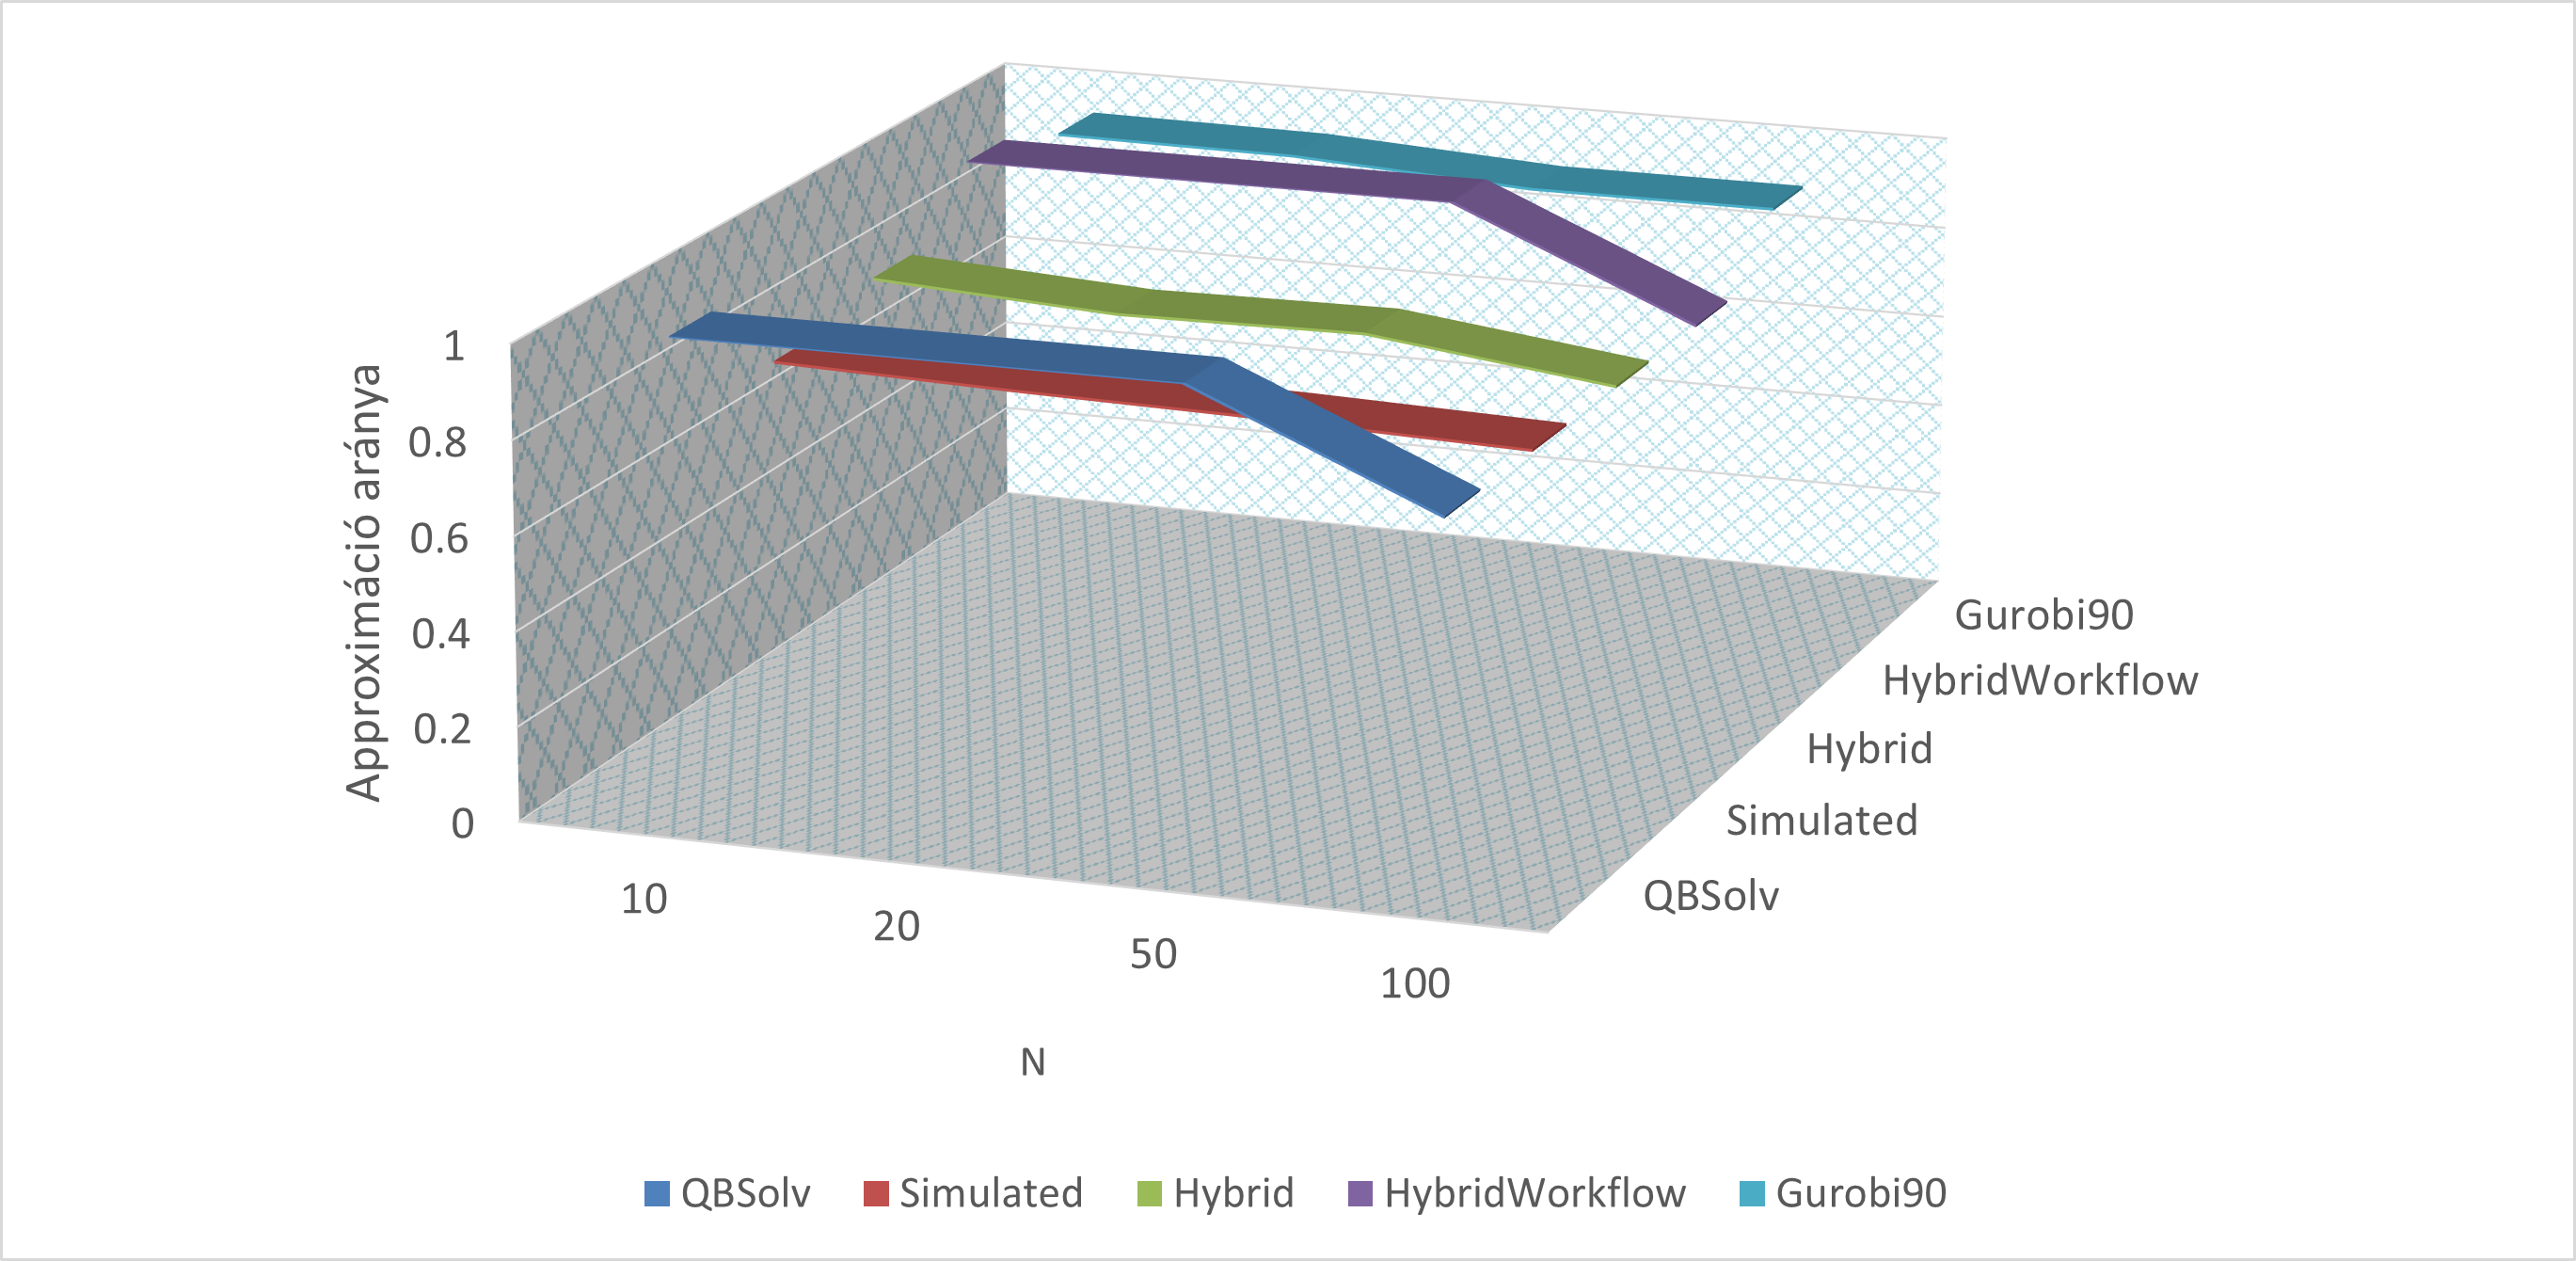
\includegraphics[width=150mm, keepaspectratio]{figures/diagrams/maxKCutQUBO_K4approx.png}
	\caption{Approximációs faktorok a max-K-vágás QUBO megoldására (K=4)}
	\label{fig:maxKCutQUBO_K4approx}
\end{figure}

Hibrid számításnál általában valamivel jobb a eredményeket kapunk, és a HybridWorkflow volt a legmegbízhatóbb, amelyet a \refstruc{fig:maxKCutQUBO_K4approx} is mutat, de kellően nagy bemeneteket ennek a megoldónak sem sikerült kezelnie.

Azt sejtjük hogy valamilyen paraméterek konfigurálásával javítható lenne ez az eredmény, de egyelőre, a viszonylag kicsi felhasználóbázis és elérhető dokumentáció miatt nem sikerült ezt kideríteni. Az viszont sajnos kiderült, hogy ebben a formájában a megoldók nem alkalmazhatók, hiszen mint láttuk, viszonylag kicsi (néhány száz csúcsból álló) gráfokra sem adnak még jó közelítést sem.

%----------------------------------------------------------------------------
\section{Maximális K-vágás (binary encoded)}\label{sec:practiceBinary}
%----------------------------------------------------------------------------

Mivel a korábban bemutatott elmélet alapján rengeteg segédváltozó bejön, így nehéz lett volna a természetes számok halmazára leképezni az összes változót, és így felírni a mátrixot. Ezért a QUBO definiálásánál kihasználtam, hogy a defaultdict kulcsainak nemcsak egész számokat, hanem akár stringeket (pontosabban string párokat) is megadhatunk, így string-ként kezelve a változóneveket kicsit követhetőbb a folyamat. Ezáltal a kódban a csoportokat elkódoló változókat \verb+x_u_i+-vel jelöltem, melynek jelentése továbbra is, az $u$ csúcs csoportját elkódoló szám i. bitje. \verb+d_u_v_i+-vel jelöltem, hogy az $u$ és $v$ csoportját elkódoló számok i. bitje különbözik-e, illetve \verb+dtemp_u_v_i+-vel a XOR kapu használatánál szükséges segédváltozót. Ennek mintájára \verb+D_u_v+ jelöli az $u$ és $v$ különböző csoportba kerülését. Ezen kívül további változók jönnek majd be az \verb+or_gate_list+ meghívásánál, ott a függvényen belül adom hozzá a Q-hoz az új változókat, úgy hogy azok nevükben egyediek legyenek, méghozzá a kimeneti változónév mögé mindig hozzákonkatenálom, hogy a lista mely indexű elemeit állítja OR kapcsolatba.

A kód egyébként két nagyobb részből áll, egyrészt a \verb+D_u_v+ változók előállítása, másrészt a  \verb+D_u_v+ változókat össze kell szorozni a megfelelő súlyokkal(\ref{code:maxKCutQUBOBinary}.~kódrészlet).

\begin{lstlisting}[language=python,caption=Max-K-cut QUBO (bináris kódolás),label=code:maxKCutQUBOBinary]

import math

# Initialize our Q matrix
Q = defaultdict(int)

# k is the number of bits needed to write a groupnumber
k = math.ceil(math.log2(K))

# Define the D_u_v variables with constraints
for u in range(K*N):
	for v in range(u+1, K*N):
		x_ui="x_"+str(u)+"_"+str(i)
		x_vi="x_"+str(v)+"_"+str(i)
		d_uvi="d_"+str(u)+"_"+str(v)+"_"+str(i)
		dtemp_uvi="dtemp_"+str(u)+"_"+str(v)+"_"+str(i)
		xor_gate(Q,x_ui,x_vi,d_uvi,dtemp_uvi)
		listOfds.append(d_uvi)
		or_gate_list(Q, listOfds, "D_"+str(u)+"_"+str(v))

# Update Q matrix for every edge in the graph
for u, v in G.edges:
	w=G.edges[u,v]['weight']
	Q[("D_"+str(u)+"_"+str(v),"D_"+str(u)+"_"+str(v))] += -1*w

\end{lstlisting}

\subsection{Logikai kapuk megvalósítása}



A fenti módszer működéséhez azonban implementálni kell a logikai kapukat is.
Ezek az elemi kapuk esetében nem okoznak különösebb problémát, hiszen a korábbi fejezetben már megadtuk, hogy milyen együtthatókat kell használni, így az implementálásnál elég egyszerűen paraméterként átvenni egy Q objektumot, melybe a változók együtthatói elmentésre kerülnek, és magukat a változókat azonosító neveket, melyekre a logikai összefüggést alkalmazni akarjuk. A Q mátrix megfelelő mezőihez hozzáadjuk a korábban kiszámolt együtthatókat, és ezzel kész is vagyunk (\ref{code:ElementaryGates}.~kódrészlet).

\begin{lstlisting}[language=python,caption=Elemi kapuk,label=code:ElementaryGates]
	
def same(Q, in1, in2):
	Q[(in1,in2)] -= 2*p
	Q[(in1,in1)] += 1*p
	Q[(in2,in2)] += 1*p

def and_gate(Q, in1, in2, out):
	Q[(in1,in2)] += 1*p
	Q[(in1,out)] -= 2*p
	Q[(in2,out)] -= 2*p
	Q[(out,out)] += 3*p

def or_gate(Q, in1, in2, out):
	Q[(in1,in2)] += 1*p
	Q[(in1,out)] -= 2*p
	Q[(in2,out)] -= 2*p
	Q[(out,out)] += 1*p
	Q[(in1,in1)] += 1*p
	Q[(in2,in2)] += 1*p

def xor_gate(Q, in1, in2, out1, out2):
	Q[(in1,in2)] += 2*p
	Q[(in1,out1)] -= 2*p
	Q[(in2,out1)] -= 2*p
	Q[(out1,out1)] += 1*p
	Q[(in1,in1)] += 1*p
	Q[(in2,in2)] += 1*p
	Q[(out2,out2)] += 12*p
	Q[(out1,out2)] += 4*p
	Q[(in1,out2)] -= 8*p
	Q[(in2,out2)] -= 8*p
	
\end{lstlisting}

A több-bemenetű OR kapura is készítettem egy rövid függvényt, amely elvégzi az OR műveletet az összes bemenetére. Mindezt úgy teszi, hogy közben felépít egy bináris fát OR kapukból, időközben segédváltozókat bevezetve. Implementációját tekintve "oszd meg és uralkodj" elven működik, vagyis rekurzívan meghívja saját magát a paraméterként átadott tömb első-, illetve második felére, majd a kapott eredményekre alkalmazza az OR műveletet (\ref{code:MultipleOrGates}.~kódrészlet).

\begin{lstlisting}[language=python,caption=Sokbemenetes OR kapu,label=code:MultipleOrGates]
	
def or_gate_list(Q, in1, out):
	length = len(in1)
	if (length==1):
	same(Q, in1[0], out)
	return
	
	half = length // 2
	out1 = out +"_0-" +str(half)  
	out2 = out +"_" +str(half) + "-" +str(length)
	or_gate_list(Q, in1[:half], out1)
	or_gate_list(Q, in1[half:], out2)
	or_gate(Q, out1, out2, out)
	
\end{lstlisting}

Illetve segédfüggvényként létrehoztam még egy bitenkénti XOR műveletet végző függvényt, mely csak annyit csinál, hogy a bemenetként kapott két listára elempáronként alkalmazza a korábban definiált \verb+xor_gate+ függvényt (\ref{code:XorGateList}.~kódrészlet).

\begin{lstlisting}[language=python,caption=Bitenkénti XOR művelet,label=code:XorGateList]
	
def xor_list(Q, in1, in2, out1, out2):
	for i in range(len(in1)):
		xor(Q, in1[i], in2[i], out1[i], out2[i])
	
\end{lstlisting}

\subsection{Eredmények}

Az eredmények nagyon hasonlóan alakultak, mint a \refstruc{sec:practiceBinary}ban láthattuk. A séma is megegyező, kis bemeneteket bármelyik megoldó jól tud kezelni, de nagy bemenetekre elkezd elképesztően rosszul teljesíteni. A \refstruc{sec:practiceOneHot}ban közölt ábrákkal analóg grafikonokat itt is előállítottam, melyekről jól leolvasható, hogy a megtalált vágás miként aránylik az optimumhoz (\ref{fig:maxKCutQUBO_K2approx_bin}, \ref{fig:maxKCutQUBO_K4approx_bin}), illetve az egyes szoftverek futásidejét a \refstruc{sec:practiceBinary}ban megfogalmazott QUBO-n (\ref{fig:maxKCutQUBO_K2_bin}, \ref{fig:maxKCutQUBO_K4_bin}). (Kivétel ismét persze a Gurobi, az megegyezik a korábban látott, korlátos programozási technikával, különben nem futna le kivárható időn belül.)

\begin{figure}[!ht]
	\centering
	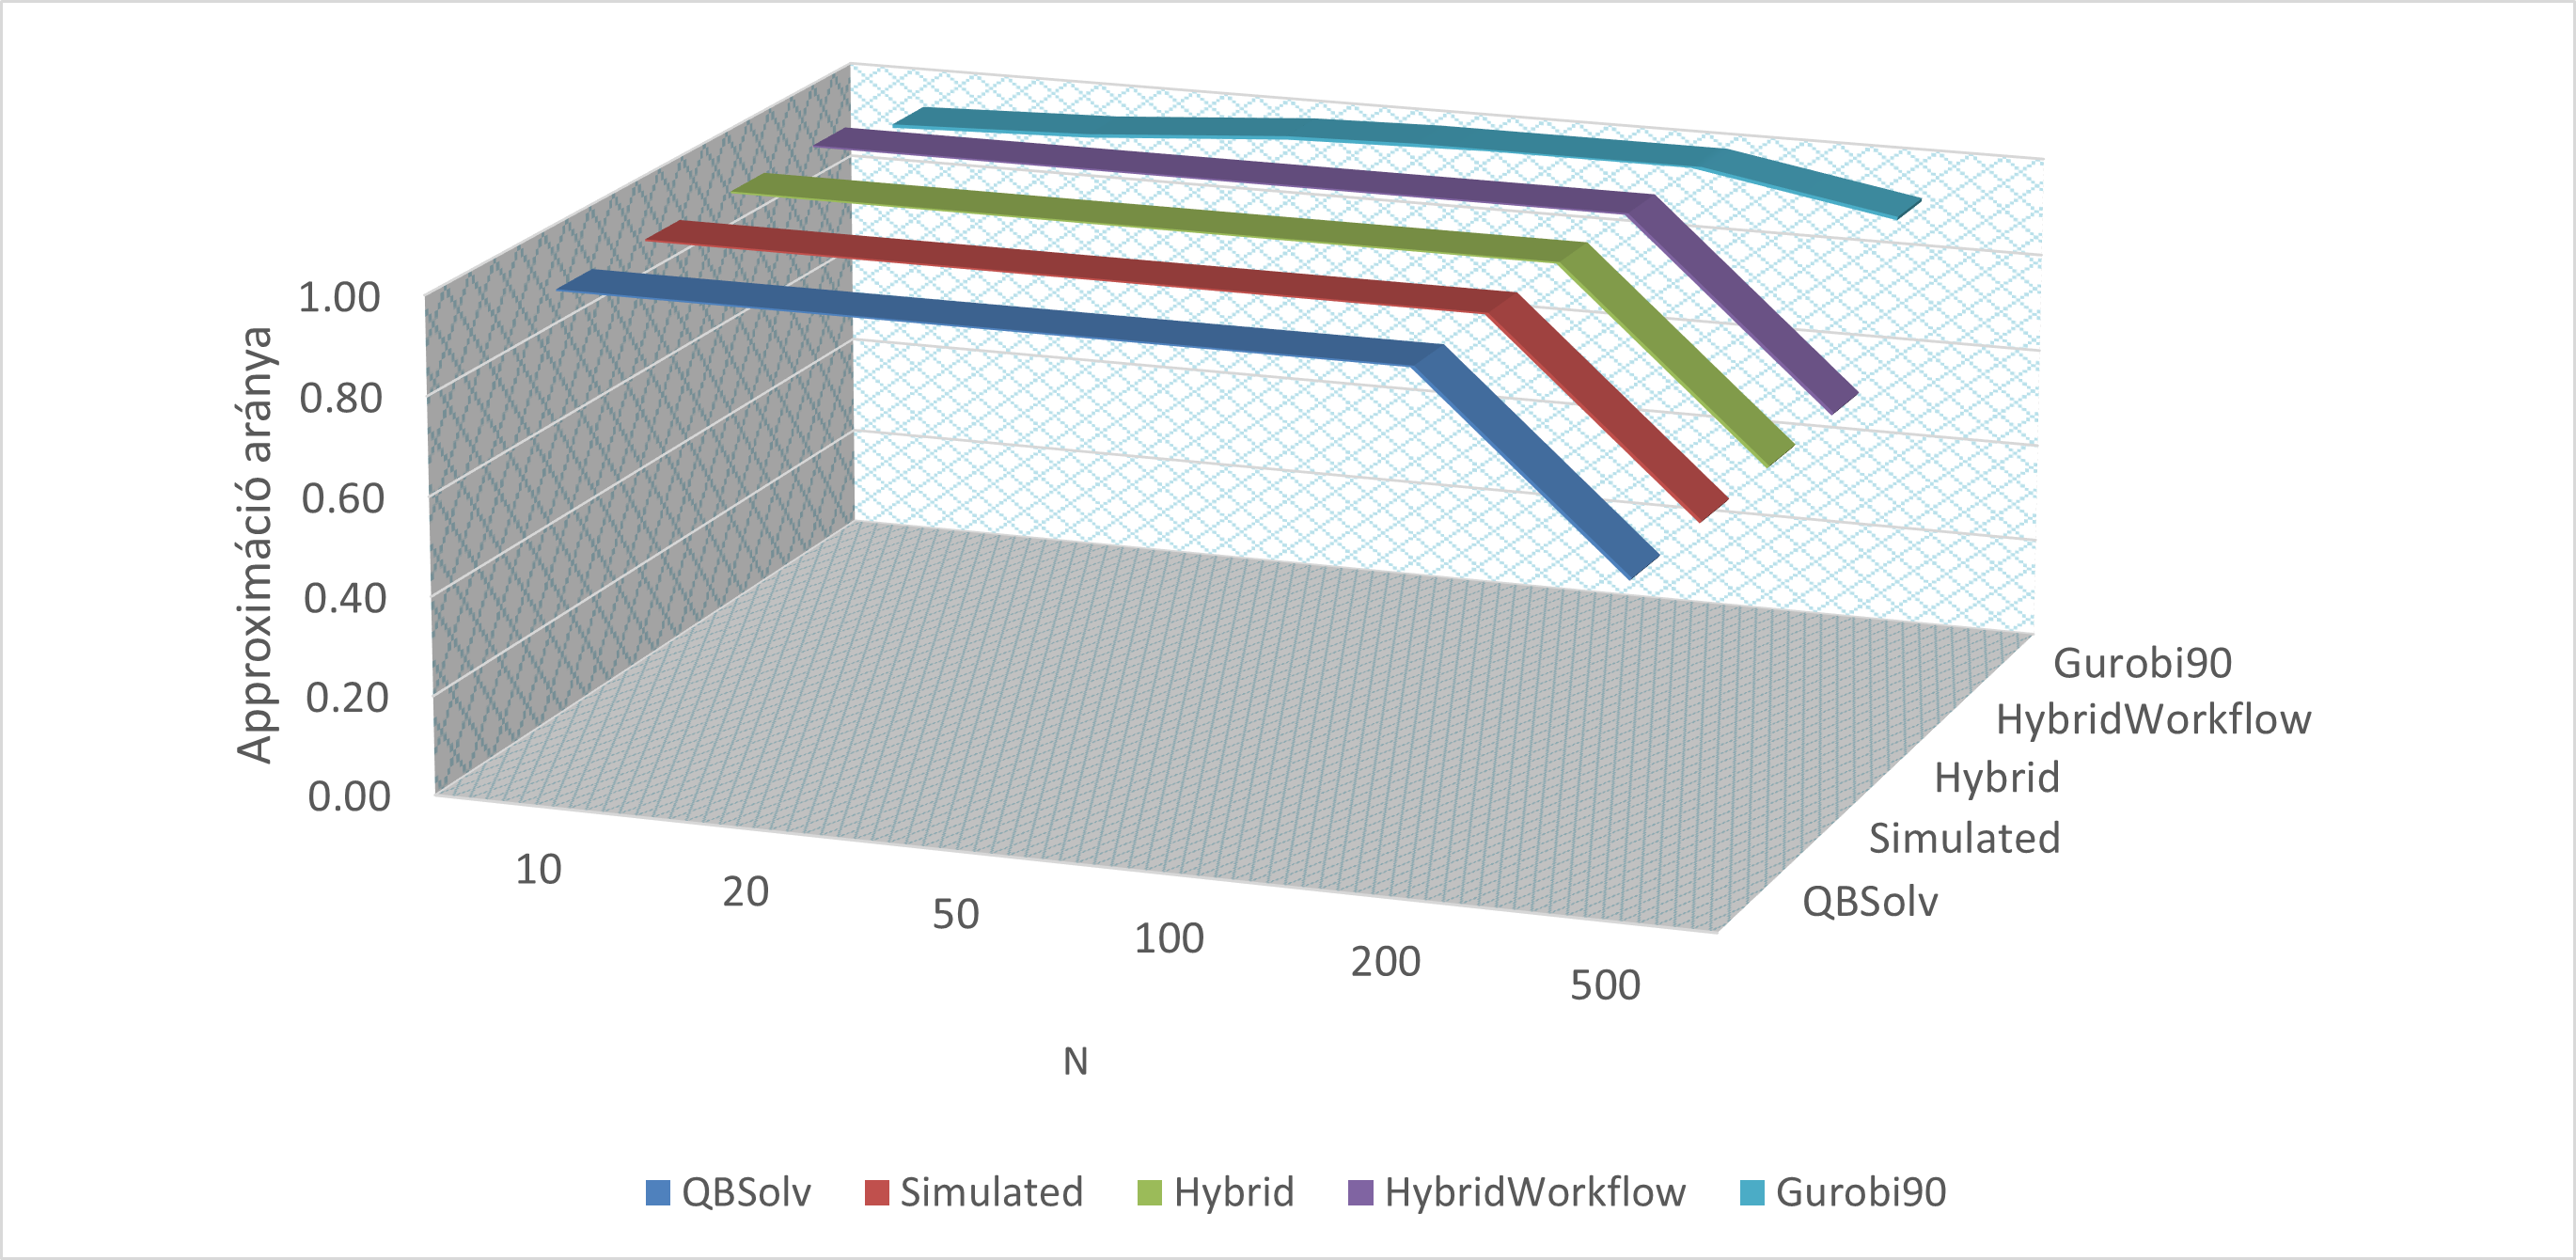
\includegraphics[width=150mm, keepaspectratio]{figures/diagrams/maxKCutQUBO_K2approx_bin.png}
	\caption{Approximációs faktorok a max-K-vágás QUBO megoldására (bináris felírás, K=2)}
	\label{fig:maxKCutQUBO_K2approx_bin}
\end{figure}

\begin{figure}[!ht]
	\centering
	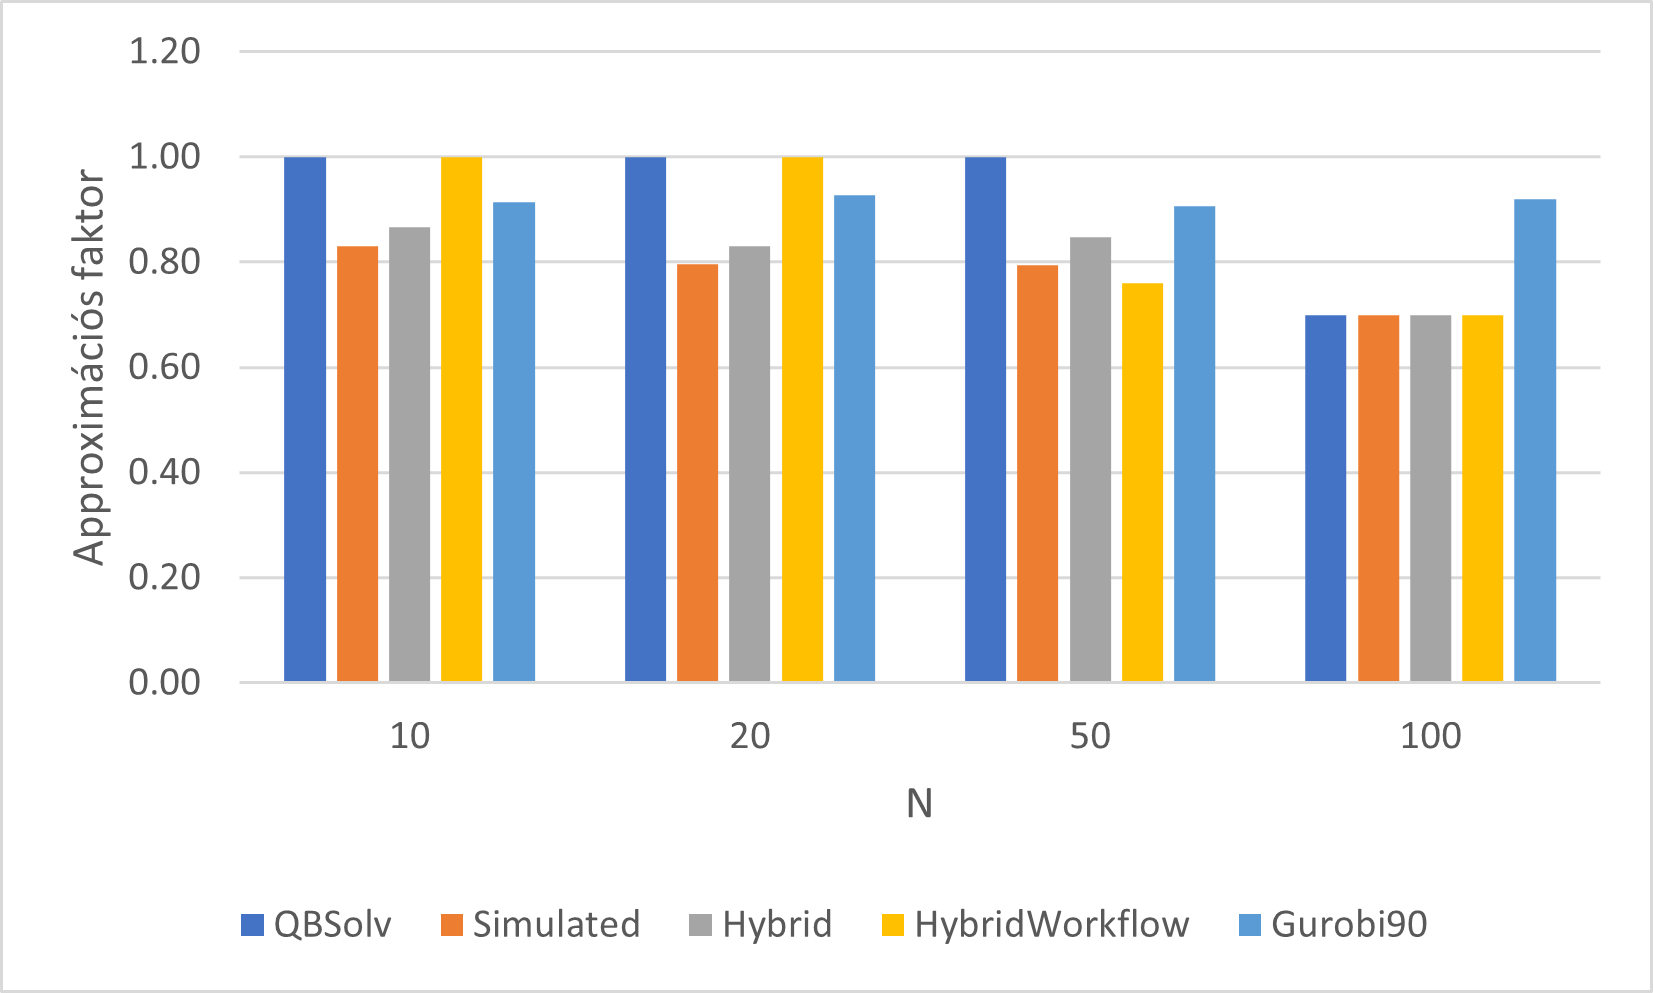
\includegraphics[width=150mm, keepaspectratio]{figures/diagrams/maxKCutQUBO_K4approx_bin.png}
	\caption{Approximációs faktorok a max-K-vágás QUBO megoldására (bináris felírás, K=4)}
	\label{fig:maxKCutQUBO_K4approx_bin}
\end{figure}

\begin{figure}[!ht]
	\centering
	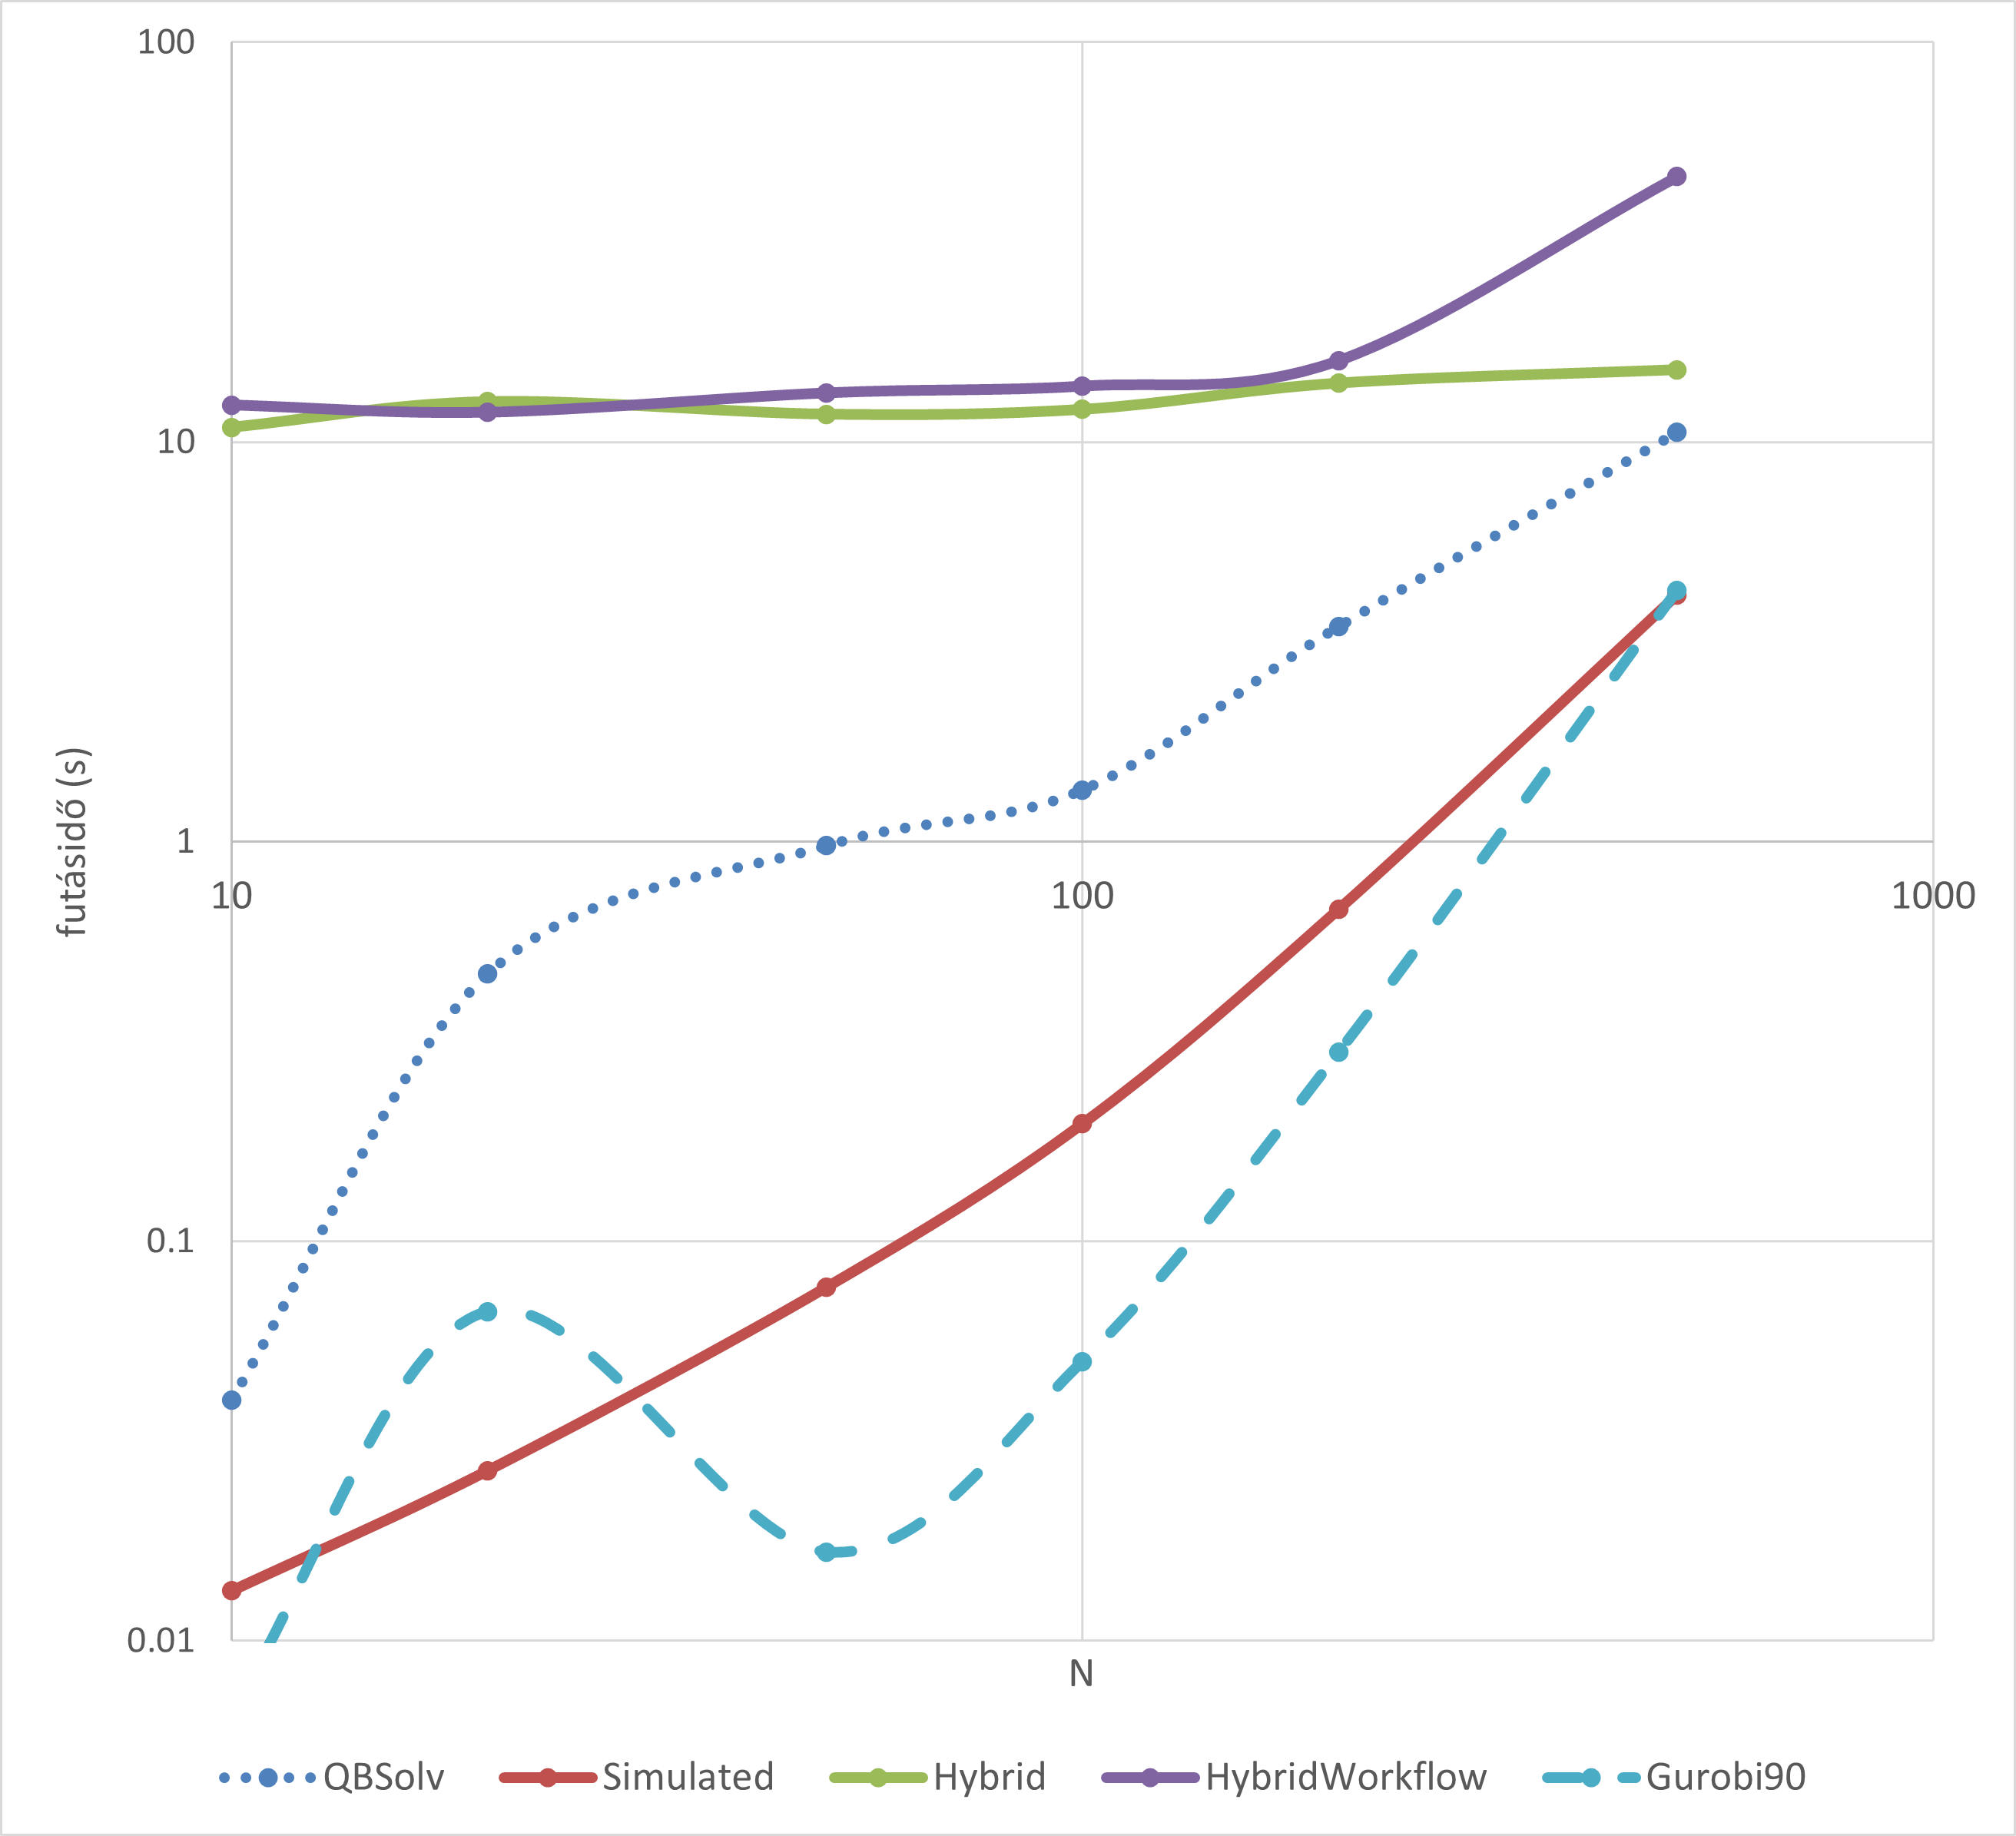
\includegraphics[width=150mm, keepaspectratio]{figures/diagrams/maxKCutQUBO_K2_bin.png}
	\caption{Futásidők a max-K-vágás QUBO megoldására (bináris felírás, K=2)}
	\label{fig:maxKCutQUBO_K2_bin}
\end{figure}

\begin{figure}[!ht]
	\centering
	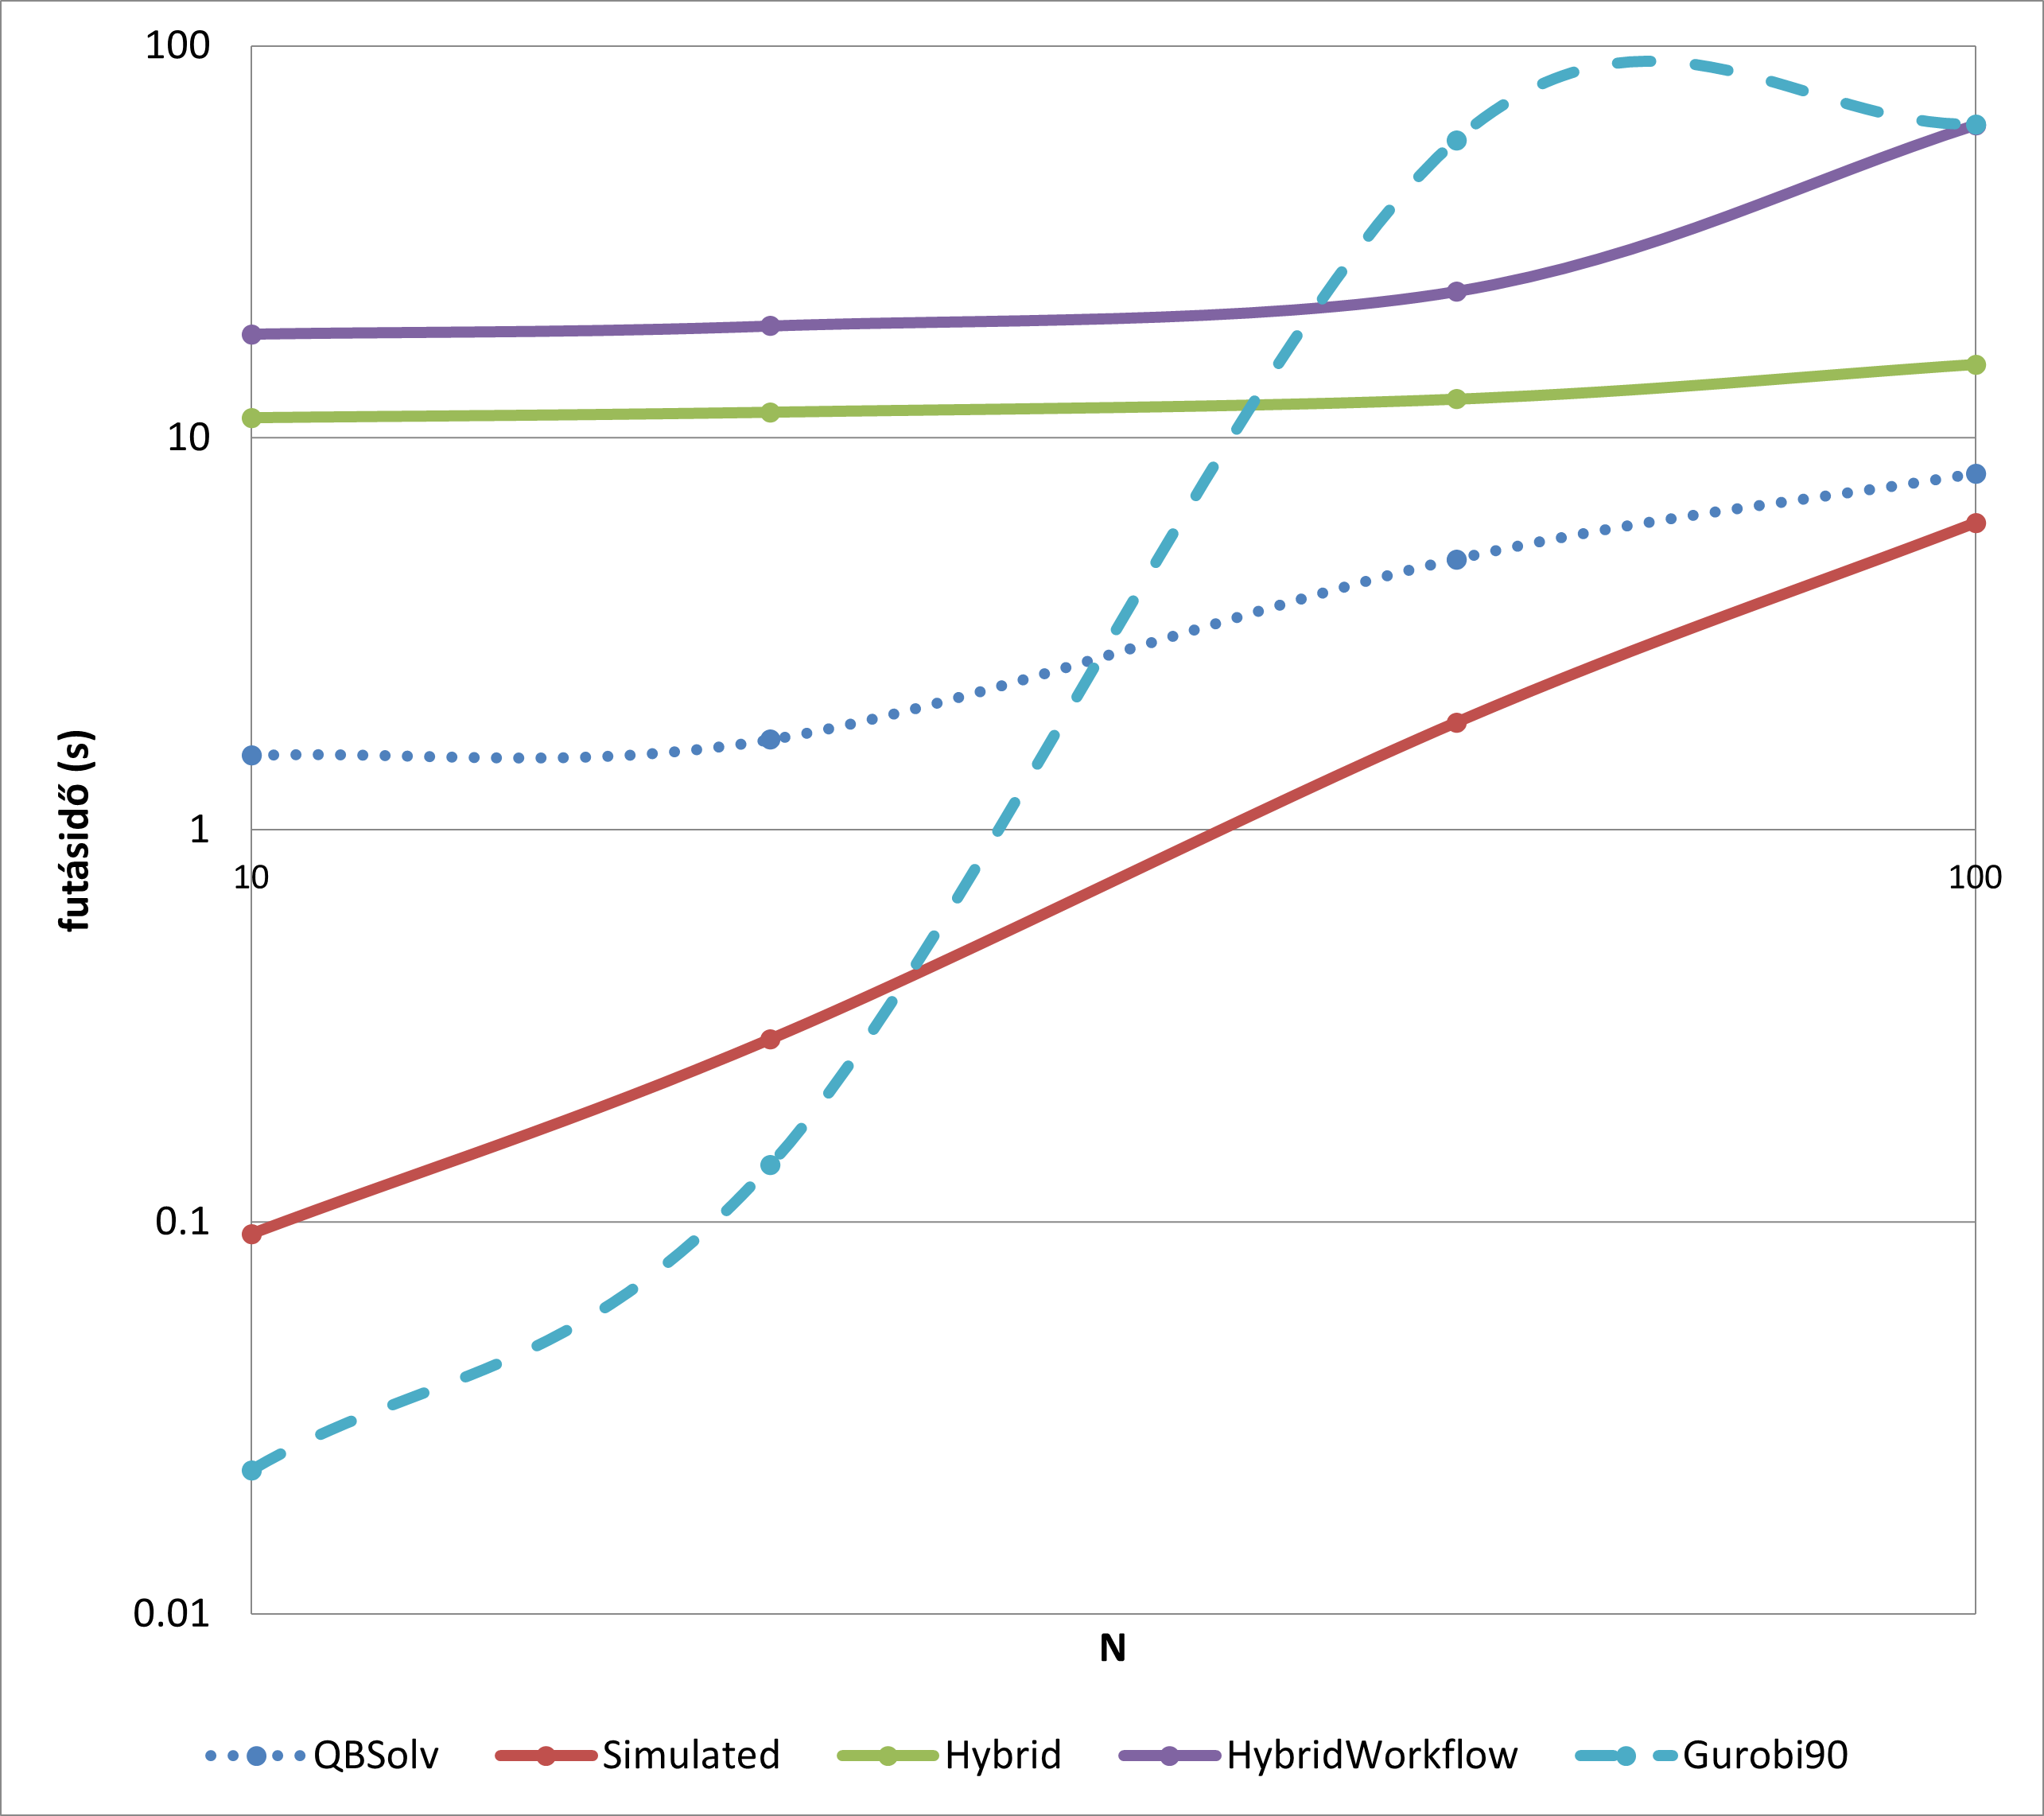
\includegraphics[width=150mm, keepaspectratio]{figures/diagrams/maxKCutQUBO_K4_bin.png}
	\caption{Futásidők a max-K-vágás QUBO megoldására (bináris felírás, K=4)}
	\label{fig:maxKCutQUBO_K4_bin}
\end{figure}